Background models are developed using the data distributions in the control region. The main sources of SM background in this analysis can be divided into 3 groups:
\begin{enumerate}
\item \textbf{Zjets events}: Zjets process is the dominating background source for this search. Lepton pairs present in the final state from the Z decay. ${p_{T}}^{miss}$ is only instrumental.
\item \textbf{Non-resonant events}: Events that have lepton pairs and ${p_{T}}^{miss}$ in the final state, while the lepton pair does not come from the decay of a resonance. $t\bar{t}$ and $WW$ processes are the main sources of the non-resonant background
\item \textbf{Resonant event}: Events that have leptons and ${p_{T}}^{miss}$ in the final state, where the lepton pair comes from the decay of a Z boson. $ZZ$ and $WZ$ are the main sources of the resonant background
\end{enumerate}

\vspace{0.3cm}
The background modeling starts from tuning the MC simulation samples. MC simulation is widely used in this analysis. The modeling of the resonant background and the signal completely rely on MC simulation. Though the modeling of the Zjet and non-resonant background are done by data-driven methods, simulation samples are also used in the process. Various weights are assigned to the MC events to compensate for discrepancies between the simulation and the actual experiment, in terms of pileup, HLT and lepton ID/Iso. The details of the background strategies for the three background groups are discussed.

\section{Pileup re-weighting}
The presence of pileup interactions can affect the quality of the event reconstruction, such as the value of ${p_{T}}^{miss}$ and lepton isolation. For the MC events, a random number of pileup interactions are added during their production, which does not necessarily agree with the pileup distribution in the data. To align the distribution of pileup interactions between data and simulation, pileup re-weighting is applied to the MC samples. 

\vspace{0.3cm}
Because the reconstruction efficiencies of the vertices might differ between MC and data, it is preferable to reweight the MC based on the distribution of the number of actual pileup interactions (true pileup), rather than observed interactions. The value of the weight assigned to the MC events is obtained from the ratio of calculated data pileup profile and the MC pileup profile. The MC pileup profile can be found in the configuration of the RunIISummer16 MC production. The calculated data pileup profile is based on the instantaneous luminosity for each bunch crossing noted in the CMS pileup JSON file, and the recommended Mini-Bias cross-section of 69.2 mb $\pm$ 4.6\% evaluated by the CMS luminosity POG.

\vspace{0.3cm}
Figure~\ref{fig:bg_pileup} shows the pileup distribution for both data and MC, as well as their ratio. The pileup reweighting value for each event in the MC samples is obtained from the ratio plot based on the pileup number in that event.

\begin{figure}[htbp]
\begin{center}
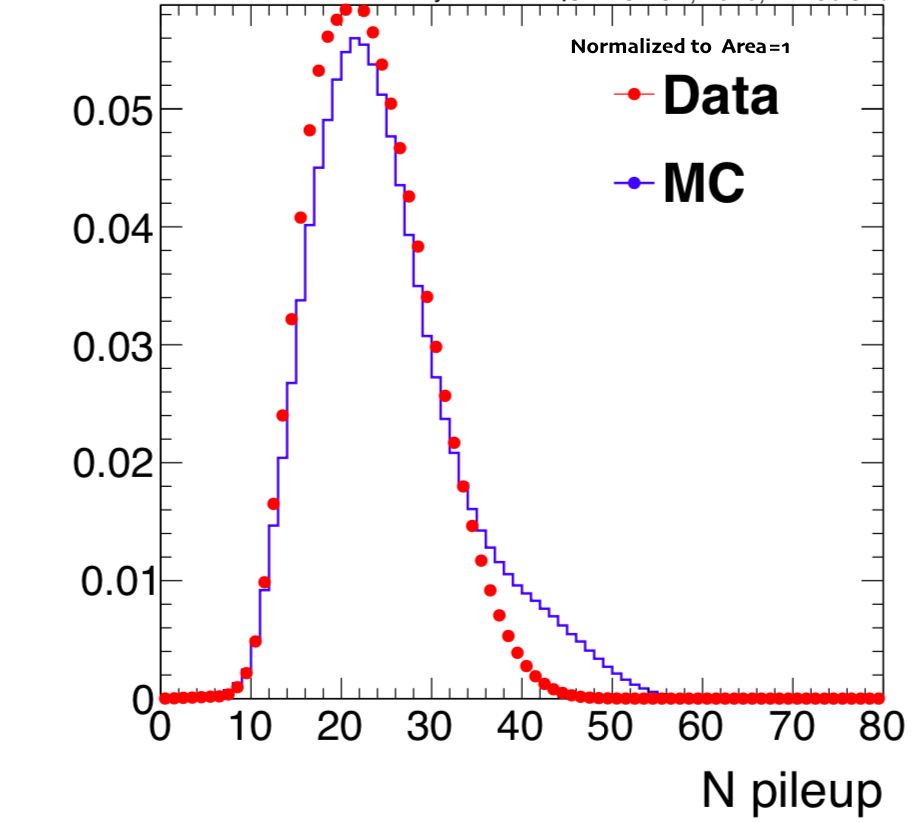
\includegraphics[width=0.45\linewidth]{figures/bg_Npileup.png}
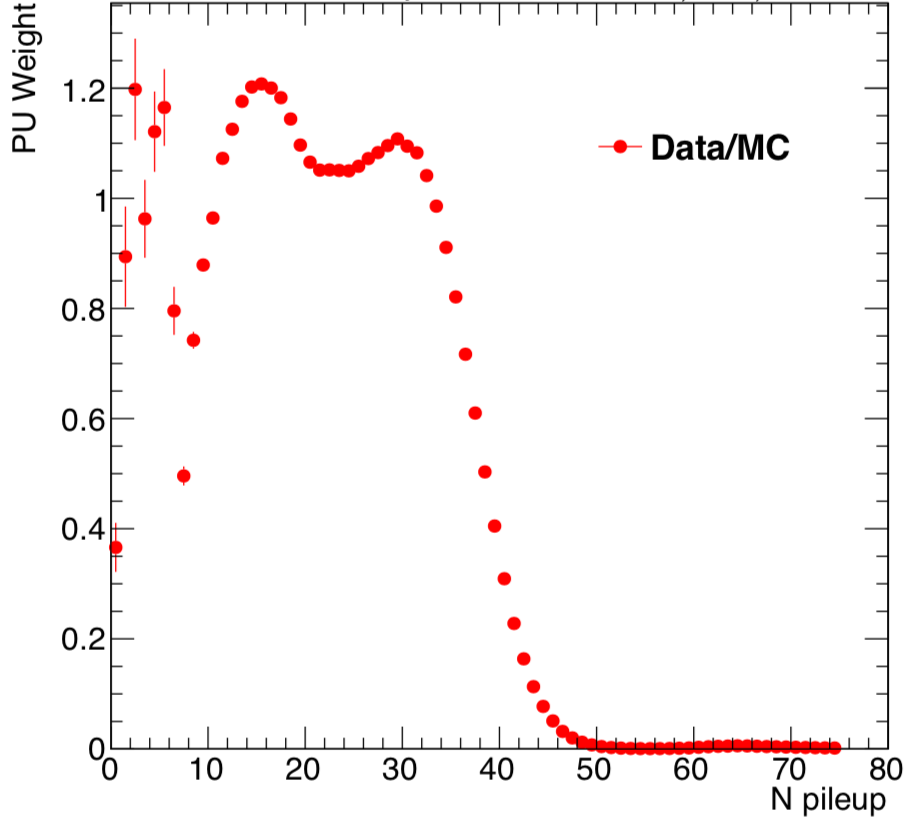
\includegraphics[width=0.45\linewidth]{figures/bg_pileupratio.png}
\caption{Pileup number profiles (left) for RunIISummer16 MC and 2016 data; and the pileup re-weighting function (right).}
\label{fig:bg_pileup}
\end{center}
\end{figure}

\section{Monte Carlo Efficiencies}
Weights are also applied to the MC samples in terms of the discrepancies in HLT and lepton ID/Iso efficiencies between data and MC samples. The probability of a lepton passing HLT, ID and Iso is:
\begin{align*}
P(HLT\cdot ID\cdot Iso) & = P(HLT|ID\cdot Iso)\times P(ID\cdot Iso) \\
 & = P(HLT|ID\cdot Iso)\times P(Iso|ID)\times P(ID),
\end{align*}
where $P(HLT\cdot ID\cdot Iso)$ denotes the efficiency of a lepton passing HLT, ID and Iso; $P(HLT|ID\cdot Iso)$ is the efficiency of a lepton passing HLT under the condition of it passing ID and ISO, and is also referred to as trigger efficiency; $P(ID\cdot Iso)$ is the combined ID/Iso efficiency; $P(Iso|ID)$ is the efficiency of a lepton passing Iso under the condition that it passes ID, referred to as the Iso efficiency; $P(ID)$ is the ID efficiency. The efficiencies are all calculated using a Tag-and-Probe method in this analysis, as discussed below. 

\subsection{Muon ID/Iso Efficiency}
The ID/Iso efficiencies may differ between MC and data due to imprecise modeling of detector performance. Therefore efficiencies are measured and scale factors (SF) are calculated for the MC samples to counter this effect. The Muon High $p_T$ ID, Tracker High $p_T$ ID and the Tracker Isolation efficiencies are measured separately using the tag-and-probe method described below. Events are selected from the SingleMuon dataset for data and DYJetsToLL\_M-50\_TuneCUETP8M1\_13TeV-madgraphMLM-pythia8 dataset for MC with pileup reweight. 

\vspace{0.3cm}
In the tag-and-probe method, a tag muon and a probe muon are selected from an event. The tag muon is a muon required to be identified with high accuracy, which helps eliminate bias, and the probe muon is the muon candidate from which the efficiency is studied. A event is kept only if two muons are found with one passing the "tag" criteria while the other passing the "probe" criteria. For the muon ID/Iso efficiency measurement, the tag criteria are:
\begin{enumerate}
\item passing the \texttt{tight} Muon ID and the $relIso<0.2$ Iso requirement recommended by CMS Muon POG
\item passing \texttt{HLT\_IsoMu24} and $p_T > 26 GeV$
\end{enumerate}

The ID and Iso requirements ensure that the tag muon is a well defined muon. The \texttt{HLT\_IsoMu24} requirement is the un-prescaled HLT with lowest $p_T$ threshold in the SingleMuon dataset. Requiring the tag muon to pass this HLT assures that the selected event will be kept in the SingleMuon dataset so that the efficiencies to be measured for the probe muon would not be biased due to the dataset selection. The $p_T > 26 GeV$ requirement is added to enforce that the trigger is highly efficient for the tag muon. A muon candidate is considered as a probe if it is reconstructed as either a global muon or a tracker muon, with $p_T > 20$ GeV.

\vspace{0.3cm}
A known issue with the tracker system during Run Periods B to F caused some tracking inefficiency in the presence of heavily ionizing particles (HIPs). The effect on the muon reconstruction is found to be minor, and accounted for by calculating the data efficiency for muons separately for Runs B to F and Runs G to H. And an additional 1\% uncertainty is assigned to cover the effect of the tracking inefficiency issue on the muon reconstruction. Considering 19.71 fb$^{-1}$ in run B to F and 16.15 fb$^{-1}$ in Run G to H, a flat random number between [0,1] is generated for each MC event, and if it is larger than $19.71 fb^{-1}/(19.71 fb^{-1}+16.15 fb^{-1})=0.5496$ the scale factors calculated from the muon efficiency in Run B to F would be assigned to the event, otherwise the SFs from Run GH are assigned.

\subsubsection{Muon ID Efficiency}
In the ID efficiency measurement, any muon candidate from the object reconstruction with $p_T > 20GeV$ and $|\eta|<2.4$ (base muon selection in the analysis) could be considered as a probe muon. Invariant mass spectra of the tag-probe muon pairs are calculated for various $p_T - \eta$ bins, with each set including a spectrum for those pairs with probe muon passing the ID, while another spectrum for pairs with probe muon failing the ID. The invariant mass spectrum consists of $Z\rightarrow \mu\mu$ process and various background processes. The $Z\rightarrow \mu\mu$ events are considered signal and the probe muon in these events are true muons. In this case, the efficiency is calculated as
\begin{equation}
\epsilon=N_{signal}^{pass}/(N_{signal}^{pass}+N_{signal}^{fail}). 
\end{equation}
The spectra are fit into $signal+background$ models, and the integral of the signal shape is $N_{signal}^{pass}$ in the passing category and $N_{signal}^{fail}$ in the failing category for each bin. 

\vspace{0.3cm}
The signal function used for the fitting is the sum of 2 Voigtians. The background profile can either be RooCMSShape~\cite{bg_cmsshape} or third order Chebychev polynomial. An example of the fitting plots is given in Figure~\ref{fig:bg_tnpmuonid}, for the Tracker High $p_T$ muon ID efficiency measurement.
\begin{figure}[htbp]
\begin{center}
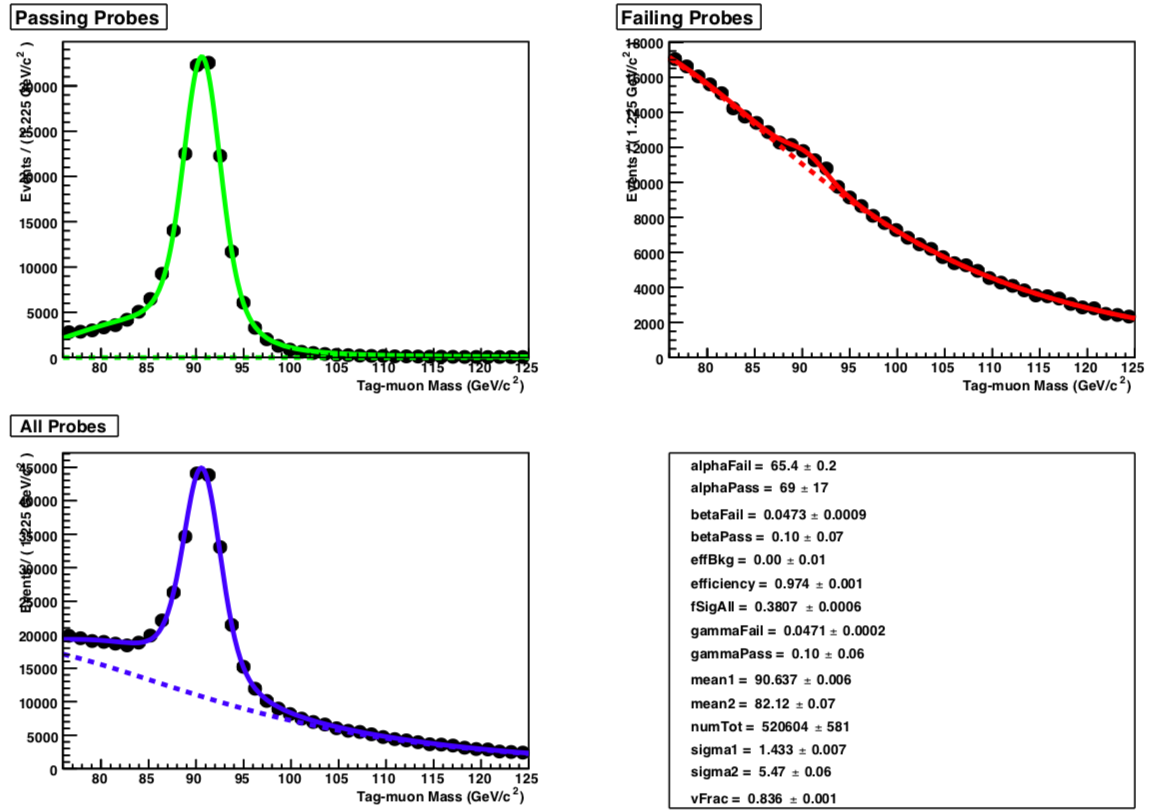
\includegraphics[width=0.9\linewidth]{figures/bg_tnpmuonid.png}
\caption{An example of the $\mu\mu$ invariant mass spectrum in one $p_T - \eta$ bin with the $signal+background$ fitting (solid lines) for the efficiency measurement of the Tracker High $p_T$ ID.} The dashed lines show the background contribution.
\label{fig:bg_tnpmuonid}
\end{center}
\end{figure}

\vspace{0.3cm}
Figures~\ref{fig:bg_muontkideff} to \ref{fig:bg_muonmcideff} show the efficiency results calculated from both Tracker High $p_T$ ID and High $p_T$ ID.

\begin{figure}[htbp]
\begin{center}
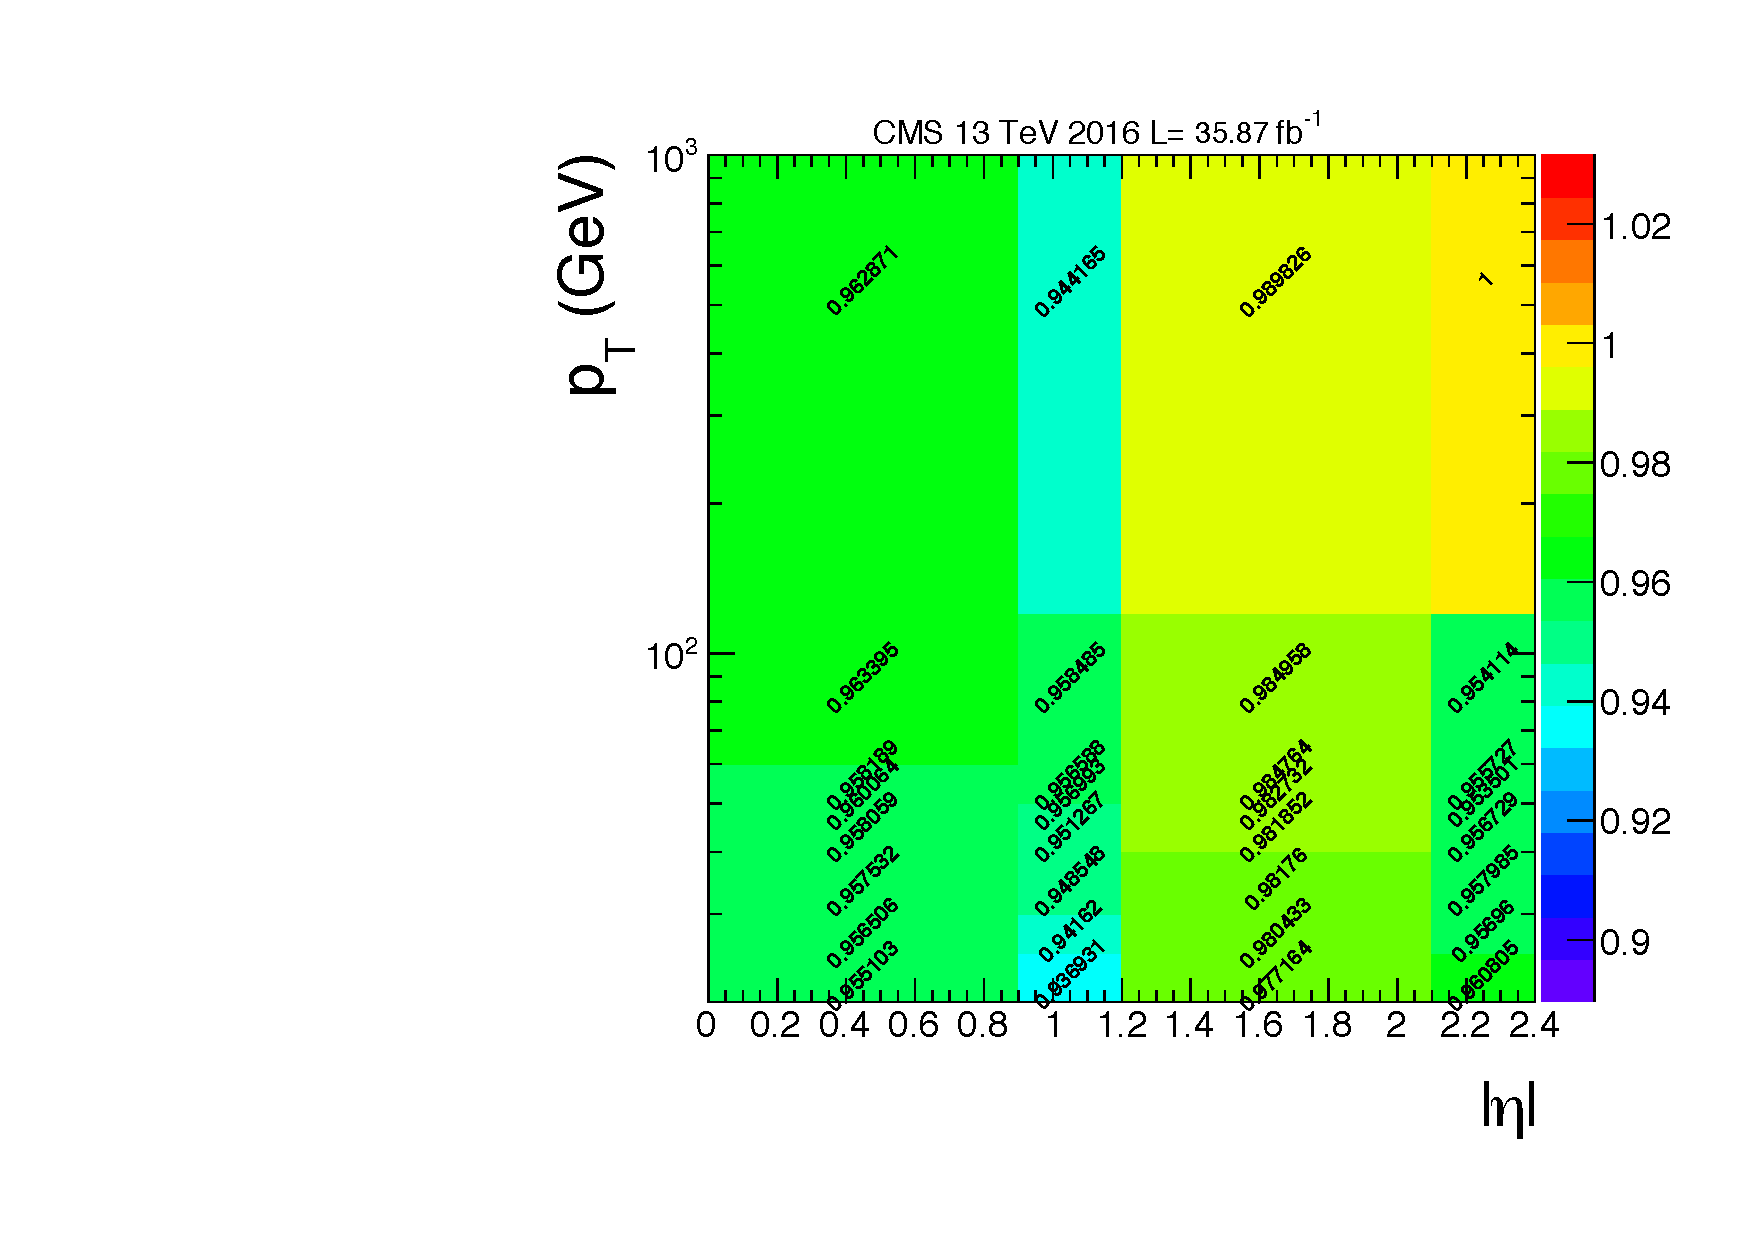
\includegraphics[width=0.49\linewidth, page=1]{figures/bg_muonidisoeff.pdf}
\includegraphics[width=0.49\linewidth, page=2]{figures/bg_muonidisoeff.pdf}
\caption{High $p_T$ Muon ID efficiency for 2016 ReReco data as a function of muon $p_T$ and $|\eta|$, for 2016 Run Peroids B--F (left) and 2016 G--H (right).}
\label{fig:bg_muontkideff}
\end{center}
\end{figure}

\begin{figure}[htbp]
\begin{center}
\includegraphics[width=0.49\linewidth, page=3]{figures/bg_muonidisoeff.pdf}
\includegraphics[width=0.49\linewidth, page=4]{figures/bg_muonidisoeff.pdf}
\caption{Tracker High $p_T$ Muon ID efficiency for 2016 ReReco data as a function of muon $p_T$ and $|\eta|$, for 2016 Run Peroids B--F (left) and 2016 G--H (right).}
\label{fig:bg_muonideff}
\end{center}
\end{figure}

\begin{figure}[htbp]
\begin{center}
\includegraphics[width=0.49\linewidth, page=5]{figures/bg_muonidisoeff.pdf}
\includegraphics[width=0.49\linewidth, page=6]{figures/bg_muonidisoeff.pdf}
\caption{Muon ID efficiency for RunIISummer16 MC as a function of muon $p_T$ and $|\eta|$, for High $p_T$ Muon ID (left) and Tracker High $p_T$ Muon ID (right).}
\label{fig:bg_muonmcideff}
\end{center}
\end{figure}

\vspace{0.3cm}
Because the Tracker High $p_T$ ID is a loosened version of the High $p_T$ ID, if a muon passes the High $p_T$ ID, it will also pass the Tracker High $p_T$ ID. The muon ID scale factor for an event is therefore calculated as:
\begin{small}
\begin{align*}
SF & =\epsilon^{data}/\epsilon^{MC} \\
 & =\frac{(\epsilon_{HighPt}(\mu_1)\times \epsilon_{trkHighPt}(\mu_2)+\epsilon_{trkHighPt}(\mu_1)\times \epsilon_{HighPt}(\mu_2)-\epsilon_{HighPt}(\mu_1)\times \epsilon_{HighPt}(\mu_2))_{data}}{(\epsilon_{HighPt}(\mu_1)\times \epsilon_{trkHighPt}(\mu_2)+\epsilon_{trkHighPt}(\mu_1)\times \epsilon_{HighPt}(\mu_2)-\epsilon_{HighPt}(\mu_1)\times \epsilon_{HighPt}(\mu_2))_{MC}}
\end{align*}
\end{small}

\subsubsection{Muon Iso Efficiency}
The muon tracker isolation efficiency is also measured using the tag-and-probe method, with an additional requirement on the probe muon to pass the tracker High $p_T$ ID. Because the tracker isolation selection applies to both muons, the ratio between the efficiencies of data and MC is used as the MC scale factor for the isolation. The SF values versus $p_T$ and $\eta$ are shown in Figure~\ref{fig:bg_muonisosf}
\begin{figure}[htbp]
\begin{center}
\includegraphics[width=0.49\linewidth, page=7]{figures/bg_muonidisoeff.pdf}
\includegraphics[width=0.49\linewidth, page=8]{figures/bg_muonidisoeff.pdf}
\caption{\texttt{tracker ISO} data/MC efficiency scale factors a function of muon $p_T$ and $|\eta|$, for 2016 Run Peroids B--F (left) and 2016 G--H (right).}
\label{fig:bg_muonisosf}
\end{center}
\end{figure}

\subsection{Electron ID/Iso Efficiency}
Based on the recommendation from the CMS EGamma POG, the \texttt{Loose} cut-based identification (ID) selection is required for all the electron candidates. Because a PF isolation is already included in the \texttt{Loose} ID, no additional electron isolation is needed.

\vspace{0.3cm}
The electron \texttt{Loose} ID (including PF ISO) efficiency and scale factors are provided by the EGamma POG, measured by the tag-and-probe method. Figure~\ref{fig:bg_eidsf} shows the electron \texttt{Loose} ID scale factors used in this analysis. The electron reconstruction is also affected by the tracking inefficiency issue, the reconstruction scale factors are also provided by the EGamma POG to counter this effect. Figure~\ref{fig:bg_gsfsf} shows the electron reconstruction scale factors from EGamma POG used in this analysis.  

\begin{figure}[htbp]
\centering
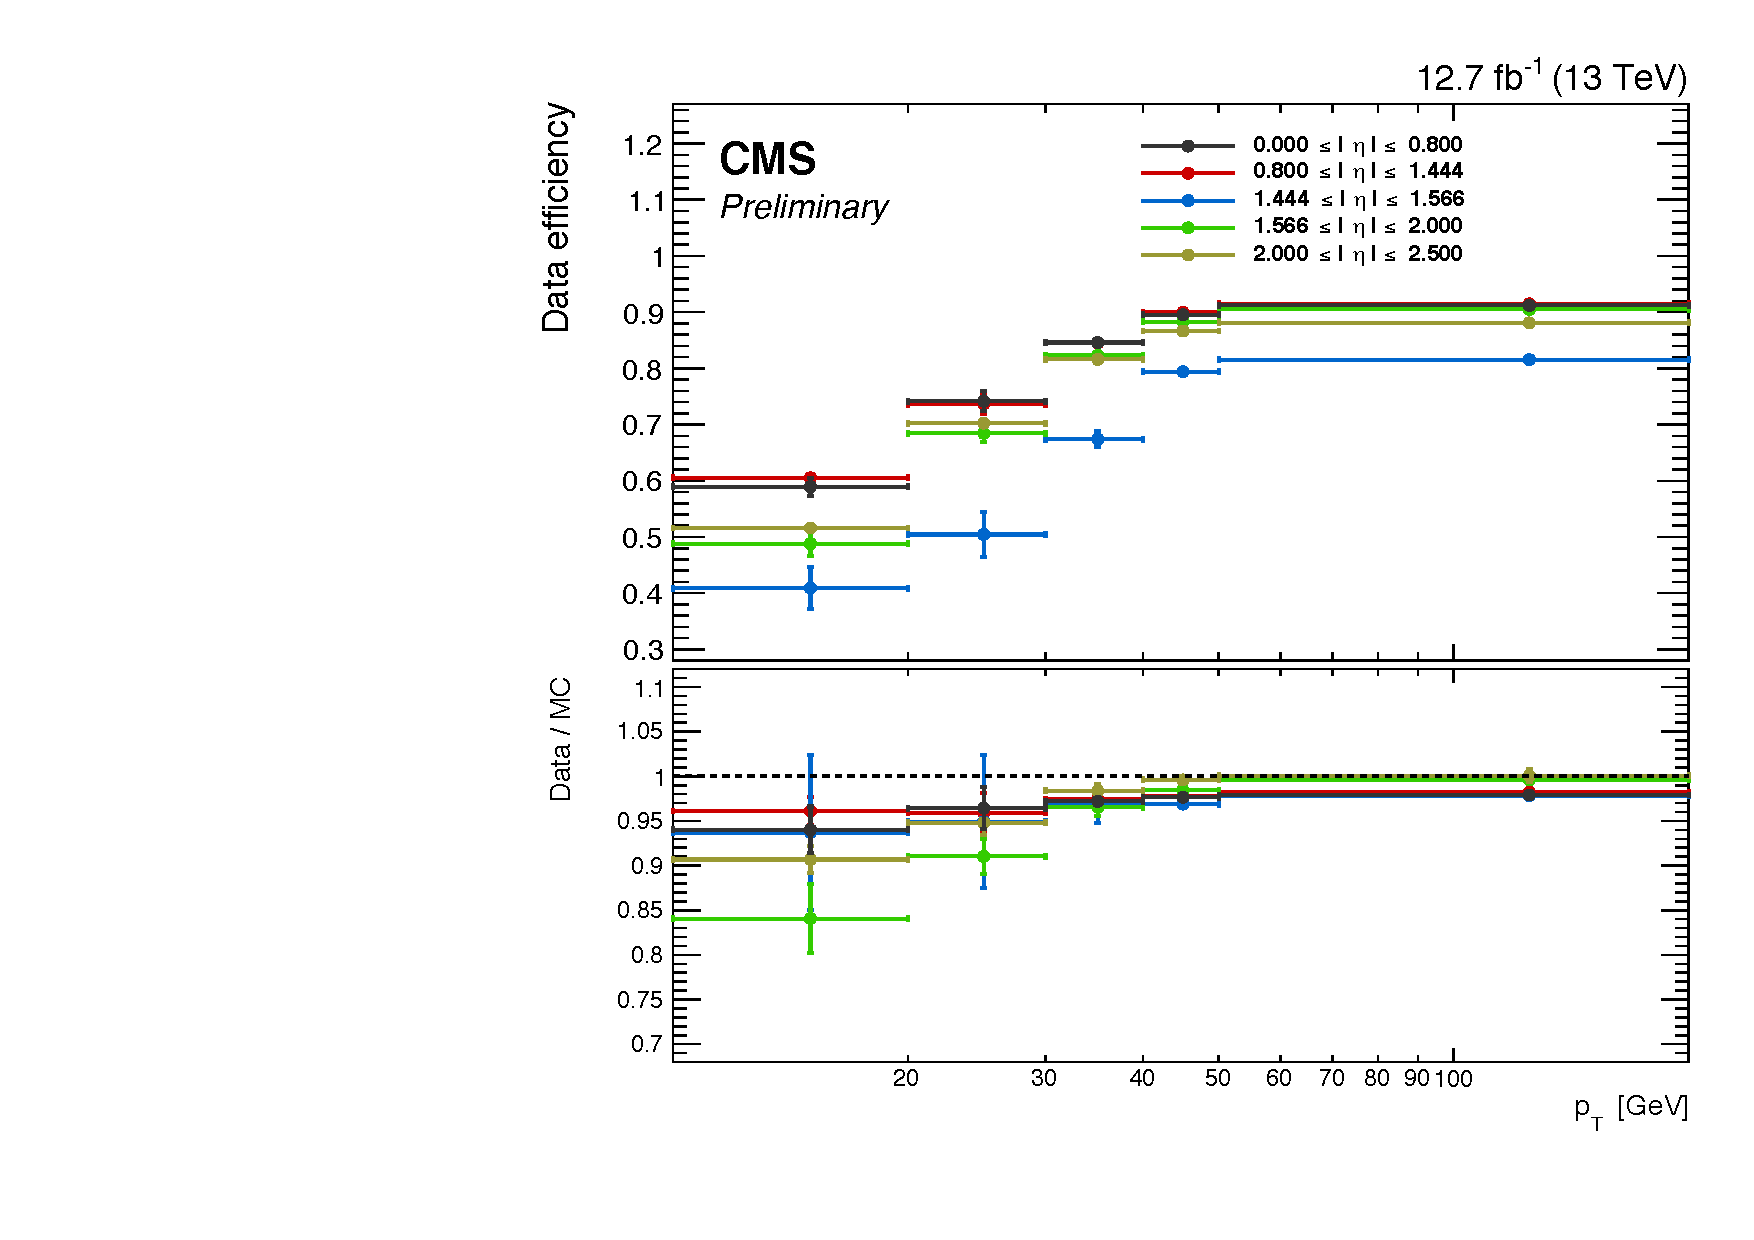
\includegraphics[width=0.66\linewidth, page=1]{figures/bg_elooseideff.pdf}
\includegraphics[width=0.66\linewidth, page=2]{figures/bg_elooseideff.pdf}
\caption{EGamma POG electron \texttt{Loose} ID (including pf Iso) efficiency scale factors for 2016 dataset analysis.}
\label{fig:bg_eidsf}
\end{figure}

\begin{figure}[htbp]
\centering
\includegraphics[width=0.66\linewidth, page=2]{figures/bg_erecoeff.pdf}
\caption{EGamma POG electron reconstruction scale factors for 2016 dataset analysis.}
\label{fig:bg_gsfsf}
\end{figure}

\subsection{Trigger Efficiency}\label{sec:bkg_trig}
The HLT is designed for making fast decisions for accepting data, and therefore the reconstruction of objects' properties at the HLT level are not as precise compared to the offline reconstruction. Trigger efficiency studies for offline objects are important to physics analyses in two regards: to suppress the trigger efficiency effect on the data by optimizing data selection; and to compensate the discrepancy in terms of trigger efficiency between data and simulation samples by applying trigger efficiency SFs to MC samples.
\subsubsection{SingleMuon HLT Efficiency}
For the muon channel selection, A event are required to pass the single muon HLT requirement of either \texttt{HLT\_Mu50} or \texttt{HLT\_TkMu50}. The combined trigger efficiencies and SFs are centrally derived by the Muon POG, measured with the tag-and-probe method. The summary plots in Figure~\ref{fig:bg_trgeff_mu} show the trigger efficiencies versus $p_T$ (left) and $\eta$ (right). In the $p_T$ plot, a rising edge of the efficiency can be clearly seen around the $p_T$ threshold of the HLT. To avoid events falling on the rising edge in the trigger efficiency, leading to greater difficulty in the background modeling, the $p_T$ of the leading muon is required to be at least 60 GeV.

\begin{figure}[htpb]
\begin{center}
\includegraphics[width=0.49\linewidth, page=2]{figures/bg_muontrgeff.pdf}
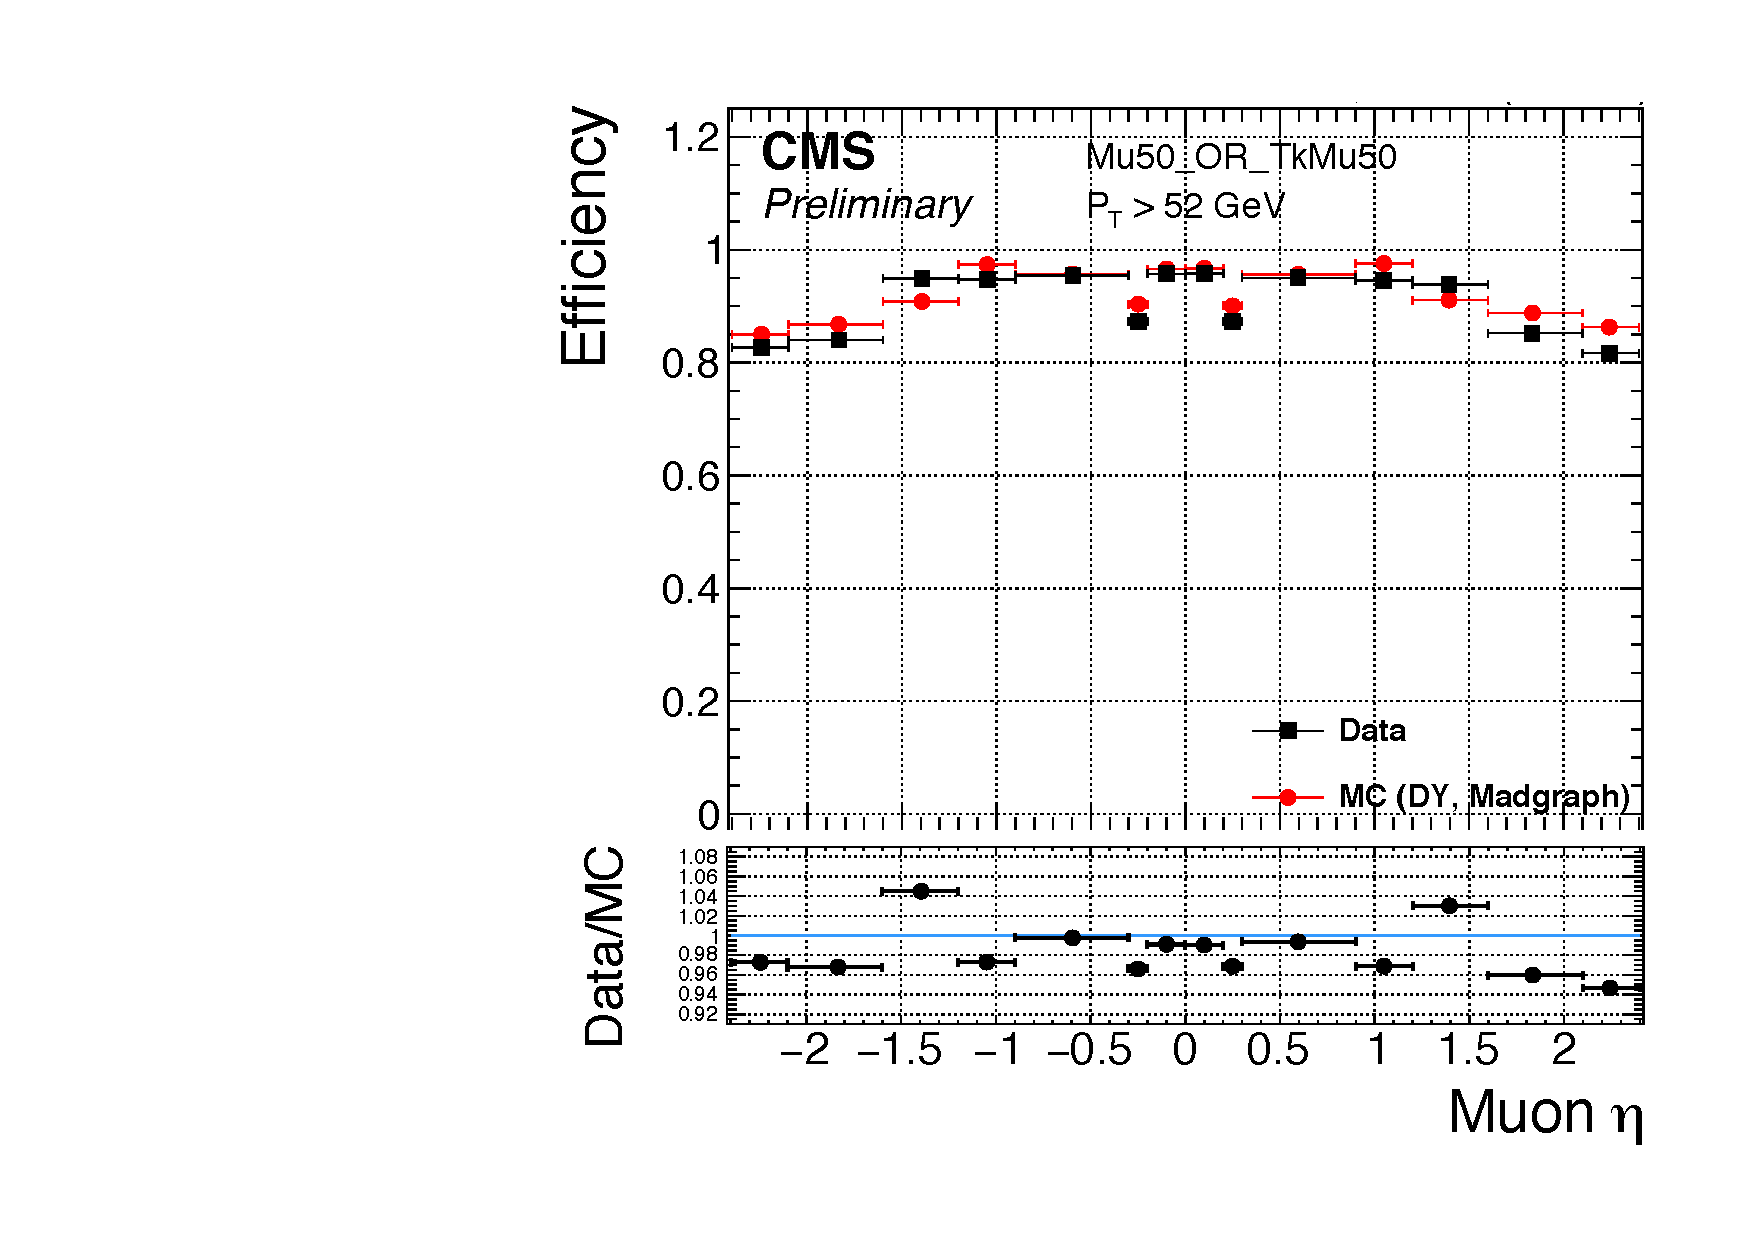
\includegraphics[width=0.49\linewidth, page=1]{figures/bg_muontrgeff.pdf}
\caption{Muon trigger efficiency for 2016 data and MC, versus $p_T$ (left) and $\eta$ (right)}
\label{fig:bg_trgeff_mu}
\end{center}
\end{figure}

\vspace{0.3cm}
The efficiency results are delivered in the form of 2D histograms in $p_T - \eta$. The calculated ratio of efficencies between data and MC are applied to the leading muon of the pair in the MC events only as the trigger efficiency scale factor, considering that number of events in either data or MC is negligible with the subleading muon passing the HLT while leading muon failing.

\subsubsection{SingleElectron HLT Efficiency}
The SingleElectron HLT (\texttt{HLT\_Ele115\_CaloIdVT\_GsfTrkIdT}) efficiency is measured for data and MC using the tag-and-probe method. Events are selected from the SingleElectron dataset in data and the DYJetsToLL\_M-50\_ TuneCUETP8M1\_13TeV-amcatnloFXFX-pythia8 dataset for MC with pileup reweight. The "tag" criteria are:
\begin{enumerate}
\item passing the \texttt{tight} cut-based identification (ID) and isolation (Iso) recommended by the EGamma POG %shown in Table~\ref{tab:electron-tightid}
\item passing \texttt{HLT\_Ele27\_WPTight\_Gsf} with $p_T>30$ and $|\eta|<2.1$
\end{enumerate}

%\begin{table}[htb!]
%  \center
%  \caption{The cuts used in the POG \texttt{tight} electron identification.}
%  \label{tab:electron-tightid}
%  \begin{tabular}{r c c c}
%    \hline
%    Variable & Barrel & Endcap \\
%    \hline
%    $|\eta_{\rm SC}|$ acceptance & $(0, 1.479)$ & $(1.479, 2.5)$\\
%    $\sigma_{i\eta,i\eta} <$ & 0.00998  & 0.0292 \\
%    $|\Delta\eta_{in}| <$ & 0.00308  & 0.00605 \\
%    $\Delta\phi_{in} <$ & 0.0816  & 0.0394 \\
%    \texttt{hOverE} $<$ & 0.0414  & 0.0641 \\
%    \texttt{relIsoWithEA} $<$ & 0.0588  & 0.0571 \\
%    $|1/E - 1/p| <$ & 0.0129  & 0.0129 \\
%    expectedMissingInnerHits $\leq$ & 1  & 1 \\
%    conversion veto & yes  & yes \\
%    \hline
%  \end{tabular}
%\end{table}

The criterion of \texttt{tight} ID/Iso ensures the tag electron to be a well identified electron. The \texttt{HLT\_Ele27\_WPTight\_Gsf} is the un-prescaled HLT with lowest $p_T$ threshold in the SingleElectron dataset, and ensures that the trigger efficiency to be measured from the probe electron is not biased due to the dataset for selection. A electron is considered as a probe if it satisfies the condition of the trigger efficiency measurement, which is passing the \texttt{loose} ID/Iso in this analysis, as described in Section~\ref{sec:ob_eidiso}.

\vspace{0.3cm}
The electron trigger efficiencies are measured as a function electron reconstructed $p_T$ and $|\eta|$ for the 2016 full dataset and RunIISummer16 MC. Figure~\ref{fig:bg_etrgtnp} gives an example of invariant mass spectrum of the electron pair. Because only electrons passing ID/Iso criteria are selected, the background fraction is very small for the trigger efficiency measurement.

\begin{figure}[htpb]
\begin{center}
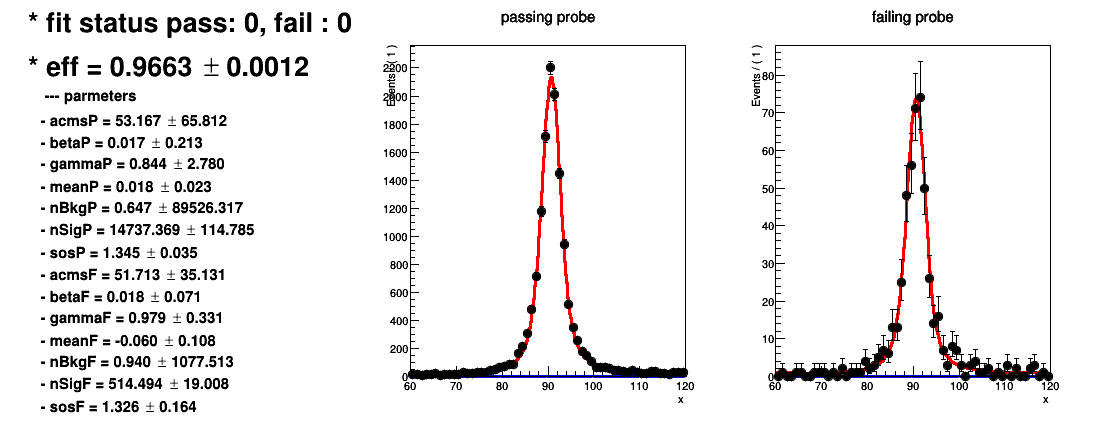
\includegraphics[width=0.95\linewidth, page=1]{figures/bg_etrgtnp.png}
\caption{An example of one  $p_T - |\eta|$ bin of the electron pair invariant mass spectrum with the $signal+background$ fitting for the efficiency measurement of \texttt{HLT\_Ele27\_WPTight\_Gsf}. The background component shown by the blue line is negligible due to the ID/Iso criteria on the probe electron.}
\label{fig:bg_etrgtnp}
\end{center}
\end{figure}

\vspace{0.3cm}
The measured efficiencies are shown in Figures ~\ref{fig:trgeff_el_dt} and \ref{fig:trgeff_el_mc} for data and MC respectively. The corresponding Data/MC scale factors are shown in Figure~\ref{fig:trgeff_el_sf}. Similar to the muon channel, the SingleElectron HLT efficiency SF is applied on the leading electron in the MC samples as reweighting factors to model the electron trigger efficiency, and a $p_T > 120$ GeV selection is added to the leading electron.

\begin{figure}[htpb]
\begin{center}
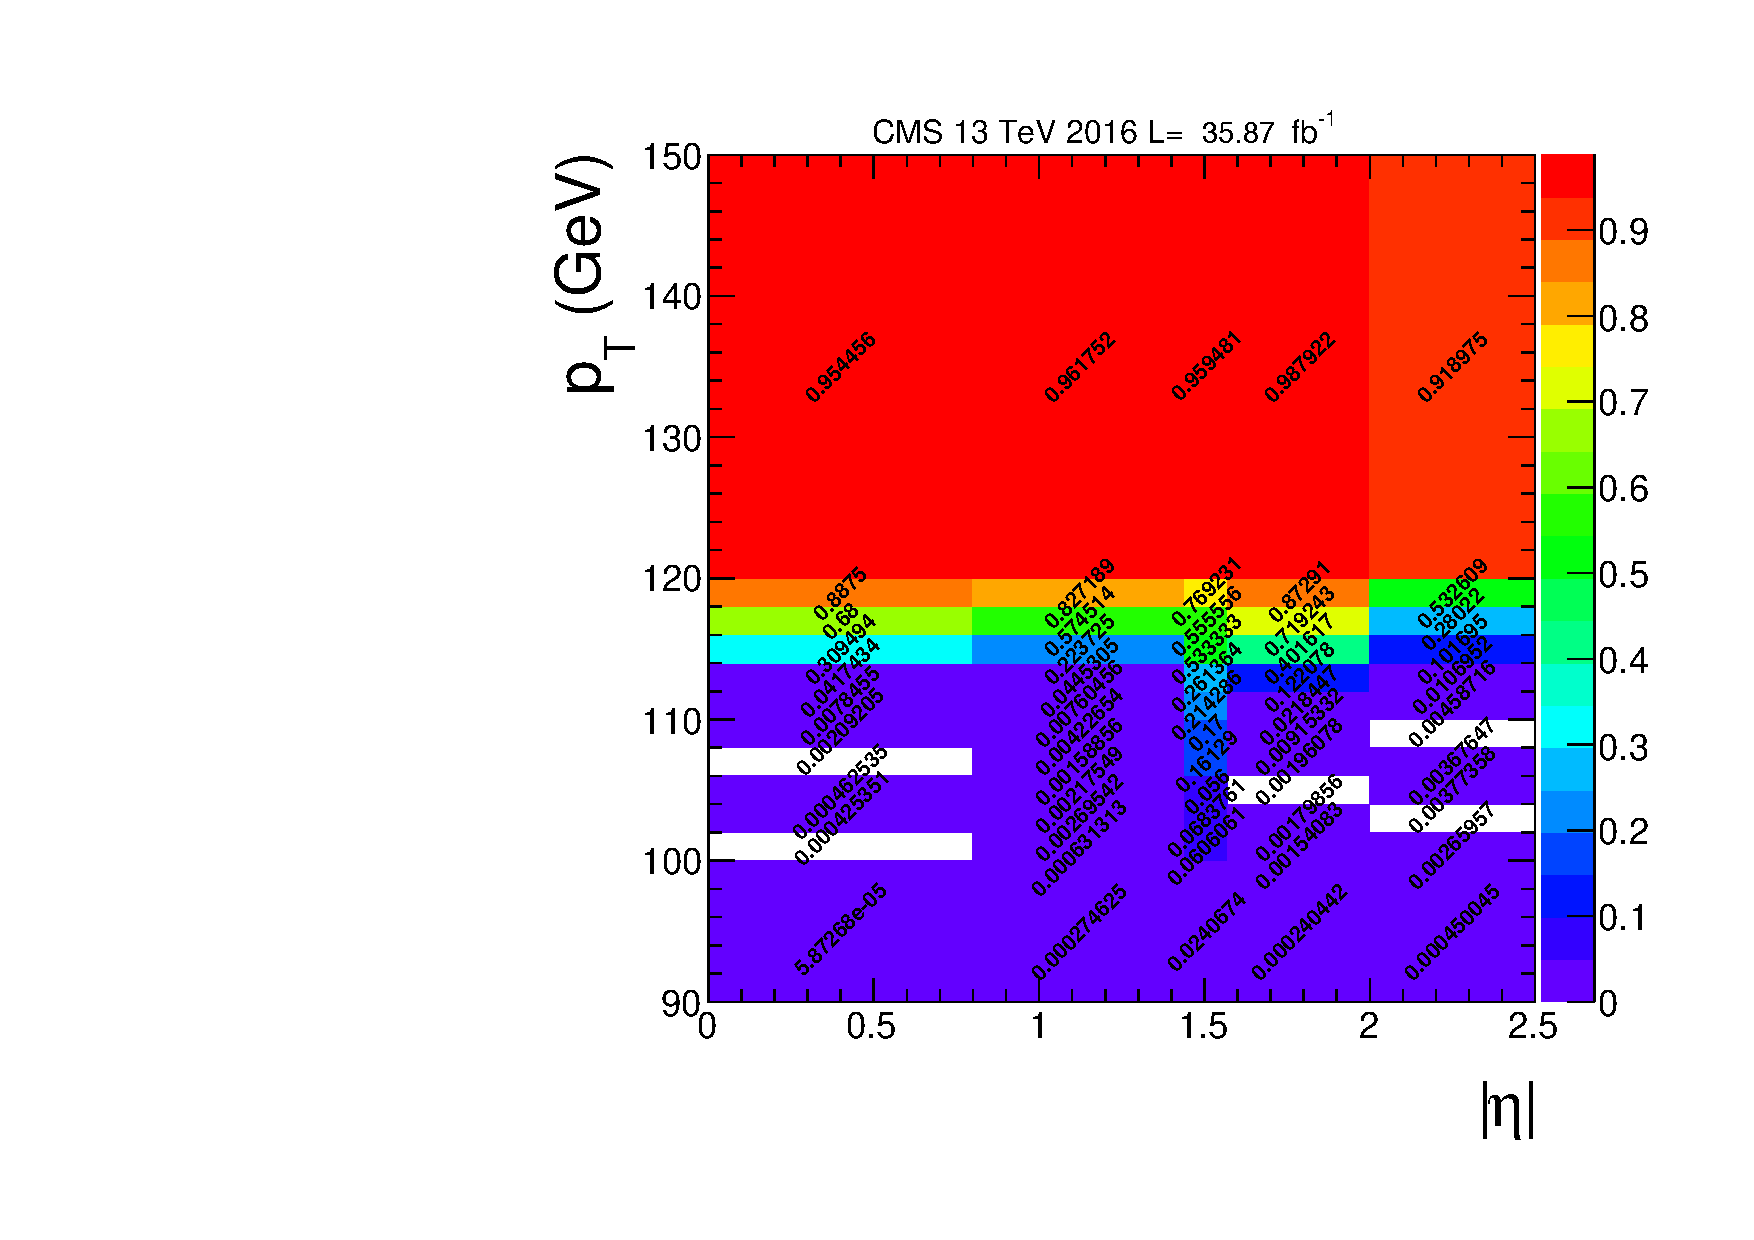
\includegraphics[width=0.49\linewidth, page=1]{figures/hlt115electron_2016fulleff_absetapt.pdf}
\includegraphics[width=0.49\linewidth, page=2]{figures/hlt115electron_2016fulleff_absetapt.pdf}
\caption{Electron trigger efficiency from 2016 ReReco dataset as a function of reconstructed electron $p_T$ and $|\eta|$. Left for $p_T <150 GeV$, right for $p_T >150GeV$. }
\label{fig:trgeff_el_dt}
\end{center}
\end{figure}

\begin{figure}[htpb]
\begin{center}
\includegraphics[width=0.49\linewidth, page=3]{figures/hlt115electron_2016fulleff_absetapt.pdf}
\includegraphics[width=0.49\linewidth, page=4]{figures/hlt115electron_2016fulleff_absetapt.pdf}
\caption{Electron trigger efficiency from RunIISummer16 MC as a function of reconstructed electron $p_T$ and $|\eta|$. Left for $p_T <150 GeV$, right for $p_T >150GeV$. }
\label{fig:trgeff_el_mc}
\end{center}
\end{figure}

\begin{figure}[htpb]
\begin{center}
\includegraphics[width=0.49\linewidth, page=5]{figures/hlt115electron_2016fulleff_absetapt.pdf}
\includegraphics[width=0.49\linewidth, page=6]{figures/hlt115electron_2016fulleff_absetapt.pdf}
\caption{Electron trigger efficiency Data/MC scale factors as a function of reconstructed electron $p_T$ and $|\eta|$. Left for $p_T <150 GeV$, right for $p_T >150GeV$. }
\label{fig:trgeff_el_sf}
\end{center}
\end{figure}

\clearpage
\section{Zjets Background Modeling}\label{sec:dybk}
In this analysis data-driven background modeling methods are used for the majority of the backgrounds, including the Zjets background. The data-driven method in this analysis has benefits in that:
\begin{enumerate}
\item The number of available MC events in the high energy region is limited, while data-driven method offers more statistics in our region of interest.
\item The modeling of ${p_{T}}^{miss}$ for the signal region is more reliable in the data-driven background methods, considering that detector conditions and pileup modeling may be imperfect in MC.
\end{enumerate}

As Figures~\ref{fig:mc_nvtx} and \ref{fig:mc_rho} show, even with the pileup reweightings applied, the vertices number and $\rho$ (a parameter describing the pileup energy in the detector) distributions still are not precisely reproduced by MC.
\begin{figure}[htbp!]
\centering
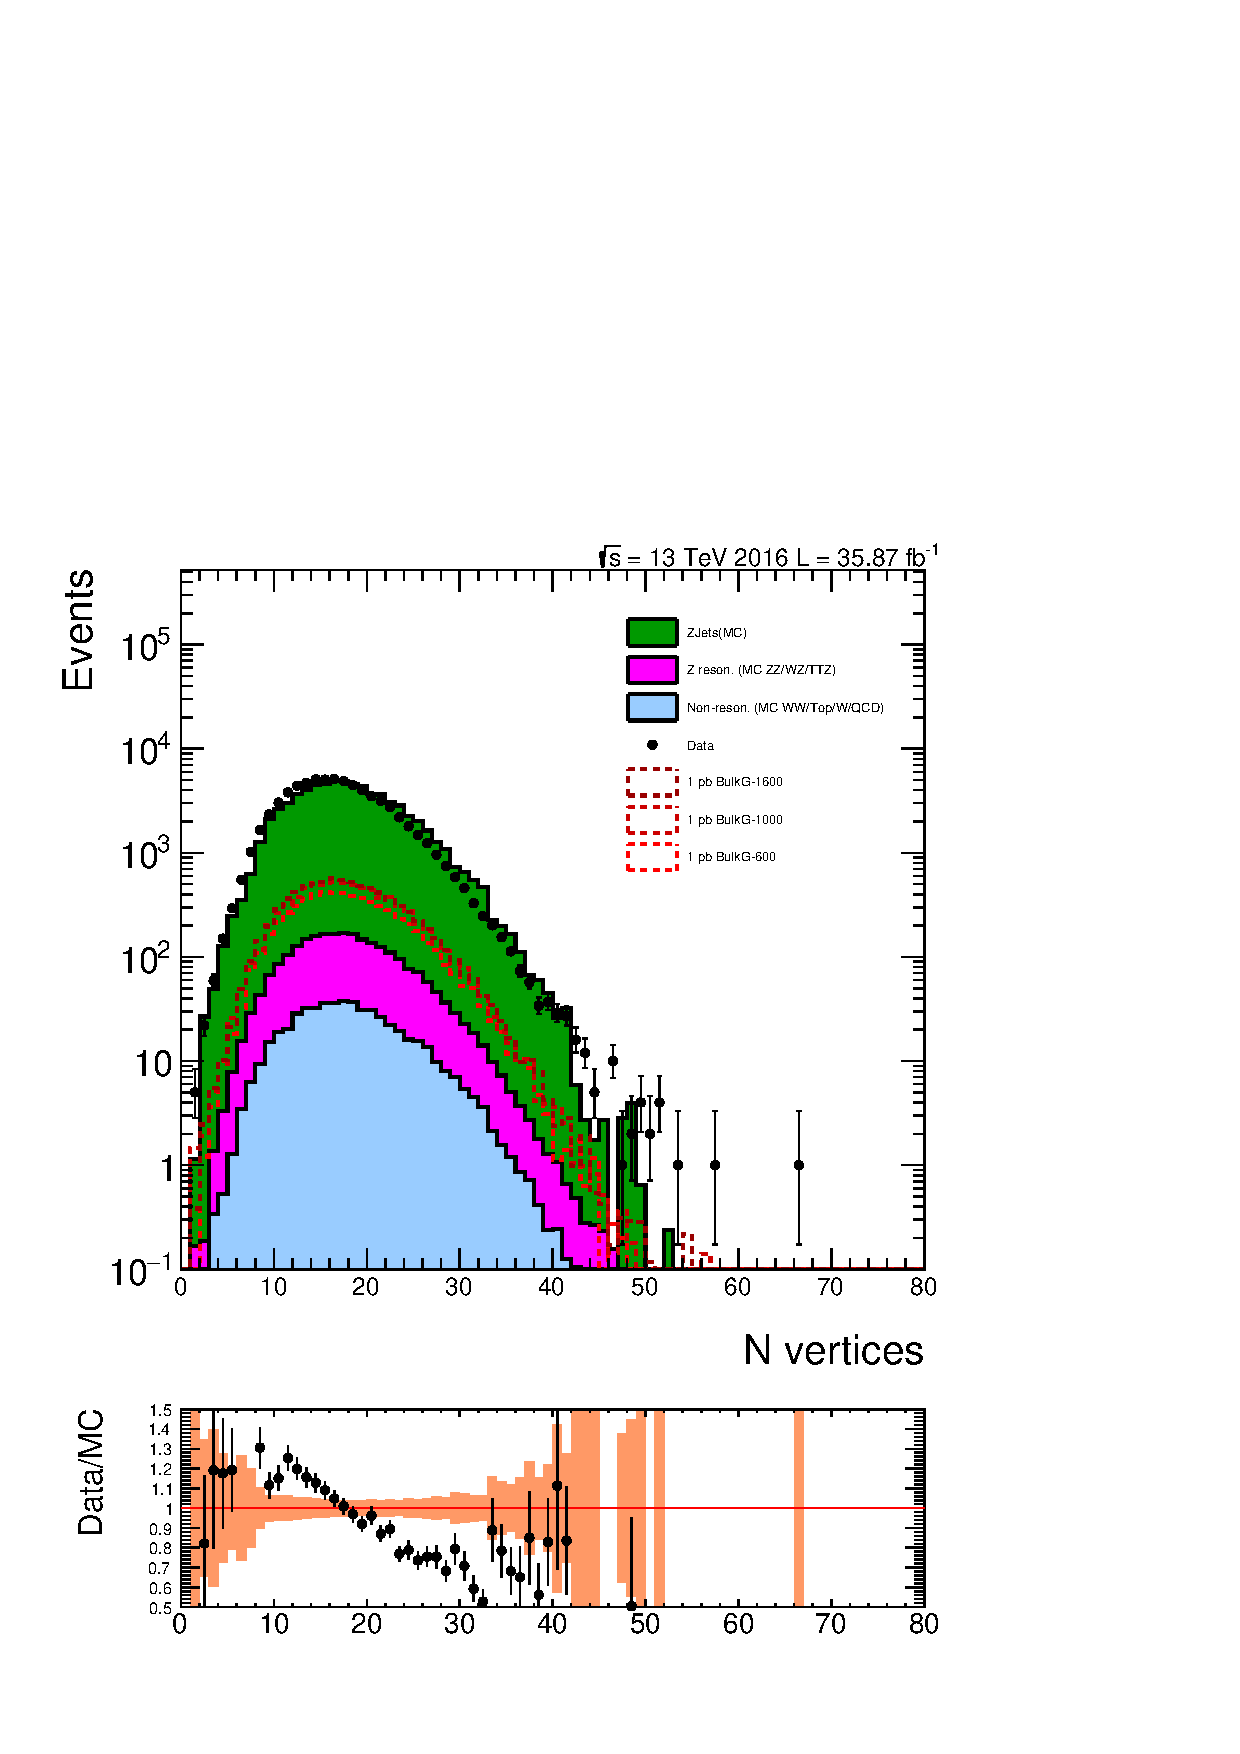
\includegraphics[width=0.46\linewidth, page=1]{figures/ReMiniSummer16_MC_GMCPhPtWt_tightzpt50_puWeightsummer16_metfilter_unblind_el_log_1pb.pdf}
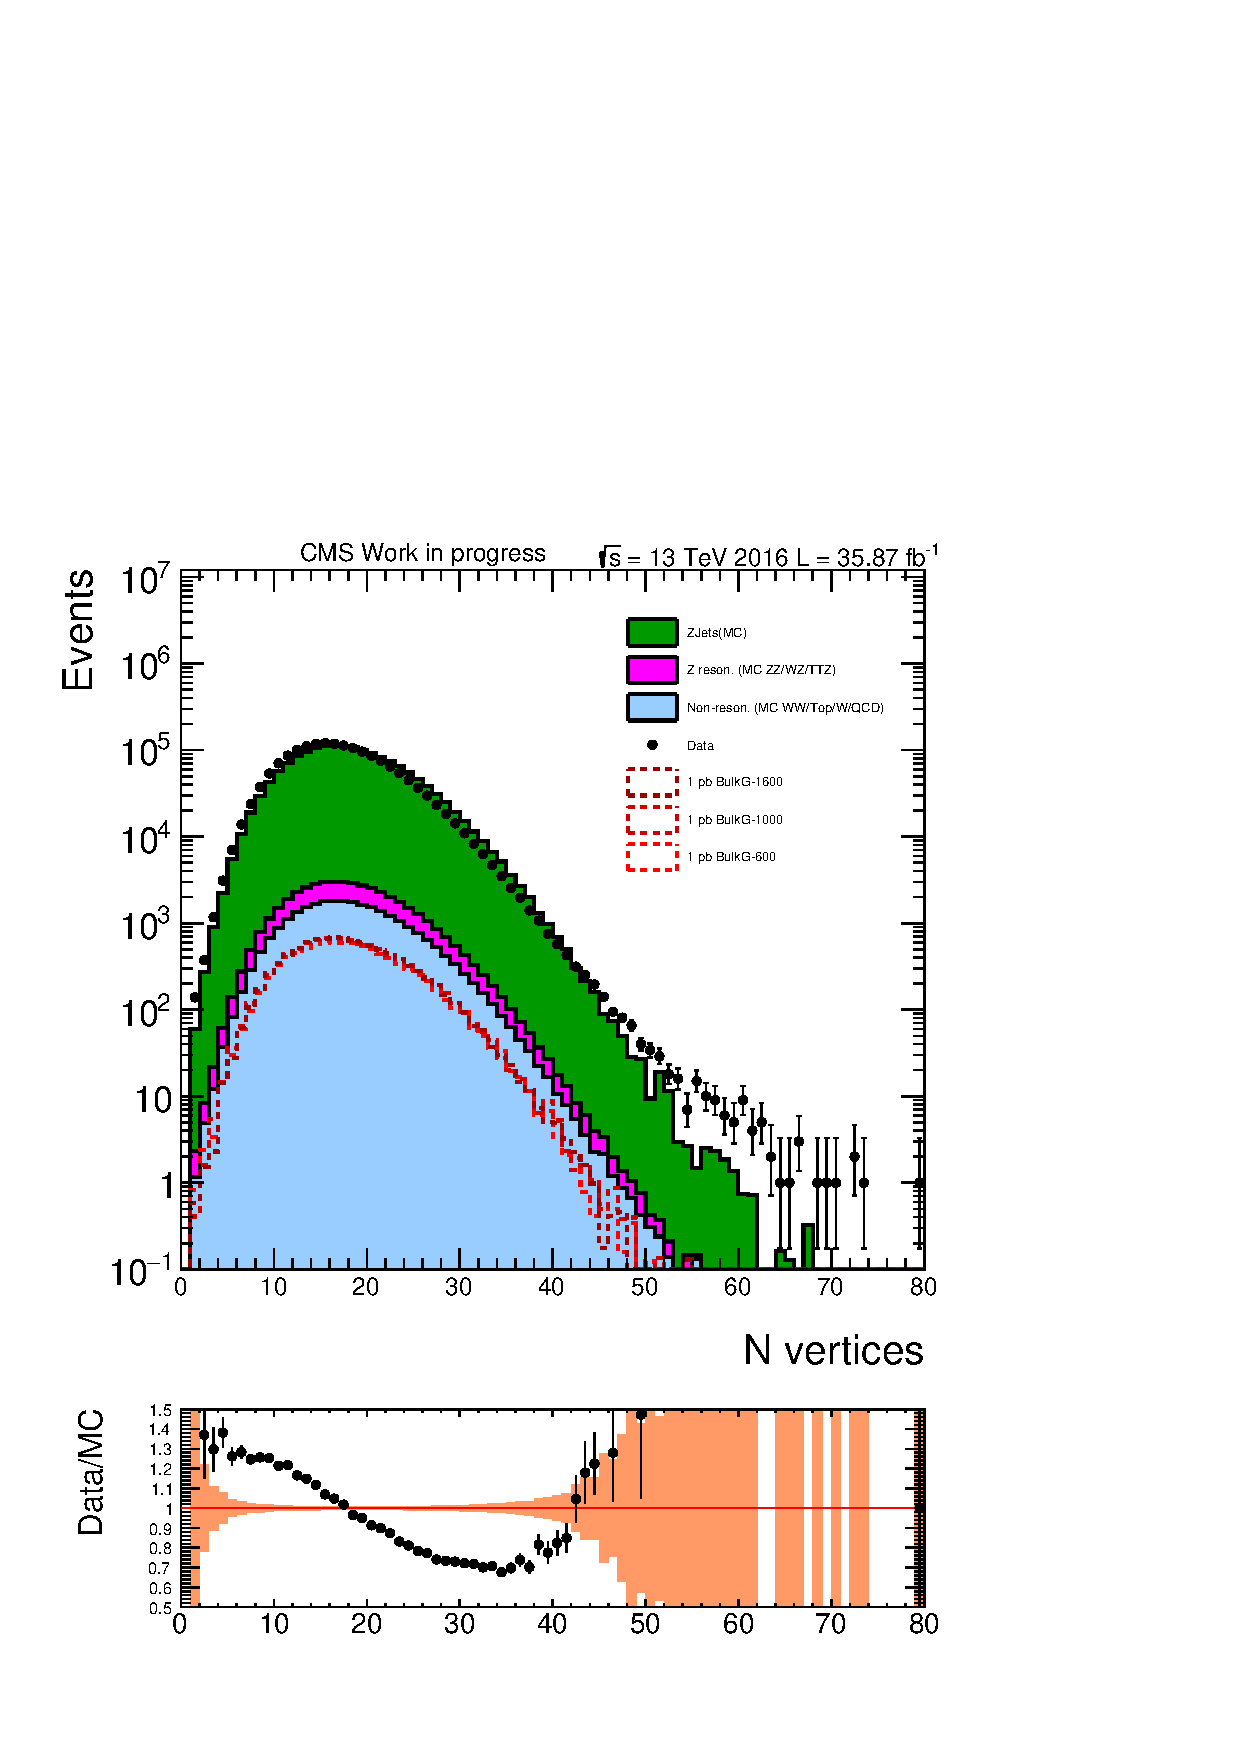
\includegraphics[width=0.46\linewidth, page=1]{figures/ReMiniSummer16_MC_GMCPhPtWt_tightzpt50_puWeightsummer16_metfilter_unblind_mu_log_1pb.pdf}
\caption{Number of reconstructed vertices for electron (left) and muon (right) channels comparing data and MC.}
\label{fig:mc_nvtx}
\end{figure}

\begin{figure}[htbp!]
\centering
\includegraphics[width=0.46\linewidth, page=2]{figures/ReMiniSummer16_MC_GMCPhPtWt_tightzpt50_puWeightsummer16_metfilter_unblind_el_log_1pb.pdf}
\includegraphics[width=0.46\linewidth, page=2]{figures/ReMiniSummer16_MC_GMCPhPtWt_tightzpt50_puWeightsummer16_metfilter_unblind_mu_log_1pb.pdf}
\caption{The $\rho$ distributions for electron (left) and muon (right) channels comparing data and MC.}
\label{fig:mc_rho}
\end{figure}

\vspace{0.3cm}
The Zjets background is characterized by a transversely boosted Z boson and a hadronic recoil balancing the momentum of the Z boson. The observed ${p_{T}}^{miss}$ in this background is completely instrumental. The photon$+$jets events have a similar kinematic signature as Zjets events, and can be used to model the Zjets background in a data-driven way. The ultimate goal would be to use the $\gamma$jets events to model the $m_T$ distribution of the Zjets background. According to Equation~\ref{eqn:intro_MTalt}, $m_T$ is determined by $m_{\ell\ell}$, ${p}_{T}^{\ell\ell}$, ${p_{T}}^{miss}_\parallel$ and ${p_{T}}^{miss}_\perp$, where $m_{\ell\ell}$ is the invariant mass of the lepton pair; ${p}_{T}^{\ell\ell}$ is the $\vec p_T$ sum of the lepton pair; ${p_{T}}^{miss}_\parallel$ refers to the projection of ${p_{T}}^{miss}$ in the direction of ${p}_{T}^{\ell\ell}$ and ${p_{T}}^{miss}_\perp$ is the fraction perpendicular to ${p}_{T}^{\ell\ell}$. It is crucial to model $m_{\ell\ell}$, ${p}_{T}^{\ell\ell}$, ${p_{T}}^{miss}_\parallel$ and ${p_{T}}^{miss}_\perp$ well. The workflow of the Zjets data-driven modeling can be summerized as below and will be discussed in the following sections:
\begin{itemize}
\item \textbf{photon data cleaning}
\begin{itemize}
\item $\gamma$jets Event Selection in Section~\ref{sec:bg_gjetsel}
\item $\gamma$jets HLT Prescale Reweighting in Section~\ref{sec:bg_gjetHLT}
\item Physical ${p_{T}}^{miss}$ Subtraction in Section~\ref{sec:bg_gjetphysmet}
\end{itemize}
\item \textbf{${p}_{T}^{\ell\ell}$ correction for photon data}
\begin{itemize}
\item ${p_T}^{\gamma}$ to ${p_T}^Z$ Reweighting in Section~\ref{sec:bg_gjetpt}
\end{itemize}
\item \textbf{$m_{\ell\ell}$ correction for photon data}
\begin{itemize}
\item Photon Mass Generation in Section~\ref{sec:gjetm}
\end{itemize}
\item \textbf{${p_{T}}^{miss}_\parallel$ and ${p_{T}}^{miss}_\perp$ corrections for photon data}
\begin{itemize}
\item ${p_{T}}^{miss}$ Hadronic Recoil Tuning in Section~\ref{sec:gjetmet}
\end{itemize}
\end{itemize}

\subsection{$\gamma$jets Event Selection}\label{sec:bg_gjetsel}
The $\gamma$jets events are selected from the SinglePhoton dataset with HLT \texttt{HLT\_Photon``PT''\_R9Id90\_HE10\_IsoM}, for \texttt{PT} = 22, 30, 36, 50, 75, 90, 120, 165 GeV. The \texttt{Loose} Photon ID defined and recommended by the CMS EGamma POG is applied. Furthermore, MET filters listed in Section~\ref{sec:metfilter} are also required in the photon data selection.

\vspace{0.3cm}
Even with the \texttt{Loose} Photon ID applied, the photons are still contaminated by many fake photons from sources such as ECAL APD spills, ECAL noise that has not been flagged, and beam halo particles. Therefore, additional selections are applied as listed below:
\begin{itemize}
\item Only one reconstructed photon in the event. 
%\item Additional fake photon events cleansing  $i\eta- i\phi$ ($ix-iy$) filter maps as shown on Figure~\ref{fig:gjets_photon_clean_eta_phi_map}. Notice that the entire region around $\phi=0$, and $\pi$ in the $x-z$ plain on the ECAL Endcap are flagged out, where beam halo photons are dominant.
\item A cleansing filter applied based on problematic ECAL channel maps.
\item \texttt{sigmaIetaIeta}$>0.001$
\item \texttt{sigmaIphiIphi}$>0.001$  
\item ``Swiss Cross'':  $S = (1-E4/E1)<0.95$ , where $E1$ is the seed crystal energy, $E4$ is the sum of the energies in up, down, left and right crystals adjacent to the seed crystal.
\item ECAL seed crystal timing :   $t_0-1.5 ns < time < t_0+1.5 ns$, where $t_0$ is the peak time position. 
\item Minimum ionizing particle (MIP) total energy $< 4.9$ GeV to suppress halo induced showers in the ECAL.
\item Lepton veto: remove events with one or more reconstructed electrons with $ p_T > 10$ GeV, 
also remove events with jets contains more than 10 GeV of lepton energy.
This is to filter out processes such as $Z\to ee$ events, with one electron mis-identified as the photon. 
\end{itemize}

In addition, analogous to the Z boson preselection, $p_T ^{\gamma} > 50GeV$ is applied in the photon data selection.

\subsection{$\gamma$jets HLT Prescale Reweighting}\label{sec:bg_gjetHLT}
Both the L1T and HLT can be prescaled in order to suppress the very high rate low energy events. For the HLTs used in the $\gamma$jets event selection:
\texttt{HLT\_Photon<$p_T$>\_R9Id90\_HE10\_IsoM}, \\
 for $p_T$ = 22, 30, 36, 50, 75, 90, 120,165 GeV:
\begin{itemize}
\item $p_T$ threshold = 165 GeV: not pre-scaled, 
\item $p_T$ threshold = 50, 75, 90, and 120 GeV:  pre-scaled at only HLT.  
\item $p_T$ threshold = 22, 30, 36 GeV: pre-scaled at both L1T and HLT, 
\end{itemize}

For photon triggers with $p_T$ of 50 GeV and higher, the L1T prescale has no effect on our selected data. The HLT prescale factor is obtained from the trigger conditions information stored for the CMS data, and applied as a weight to correct the effect of the HLT prescale on the $p_T$ spectrum of the photons. Figure~\ref{fig:photon_pt_prescale} shows the photon $p_T$ spectrum with and without corrections for the HLT prescales.


\begin{figure}[htbp]
\begin{center}
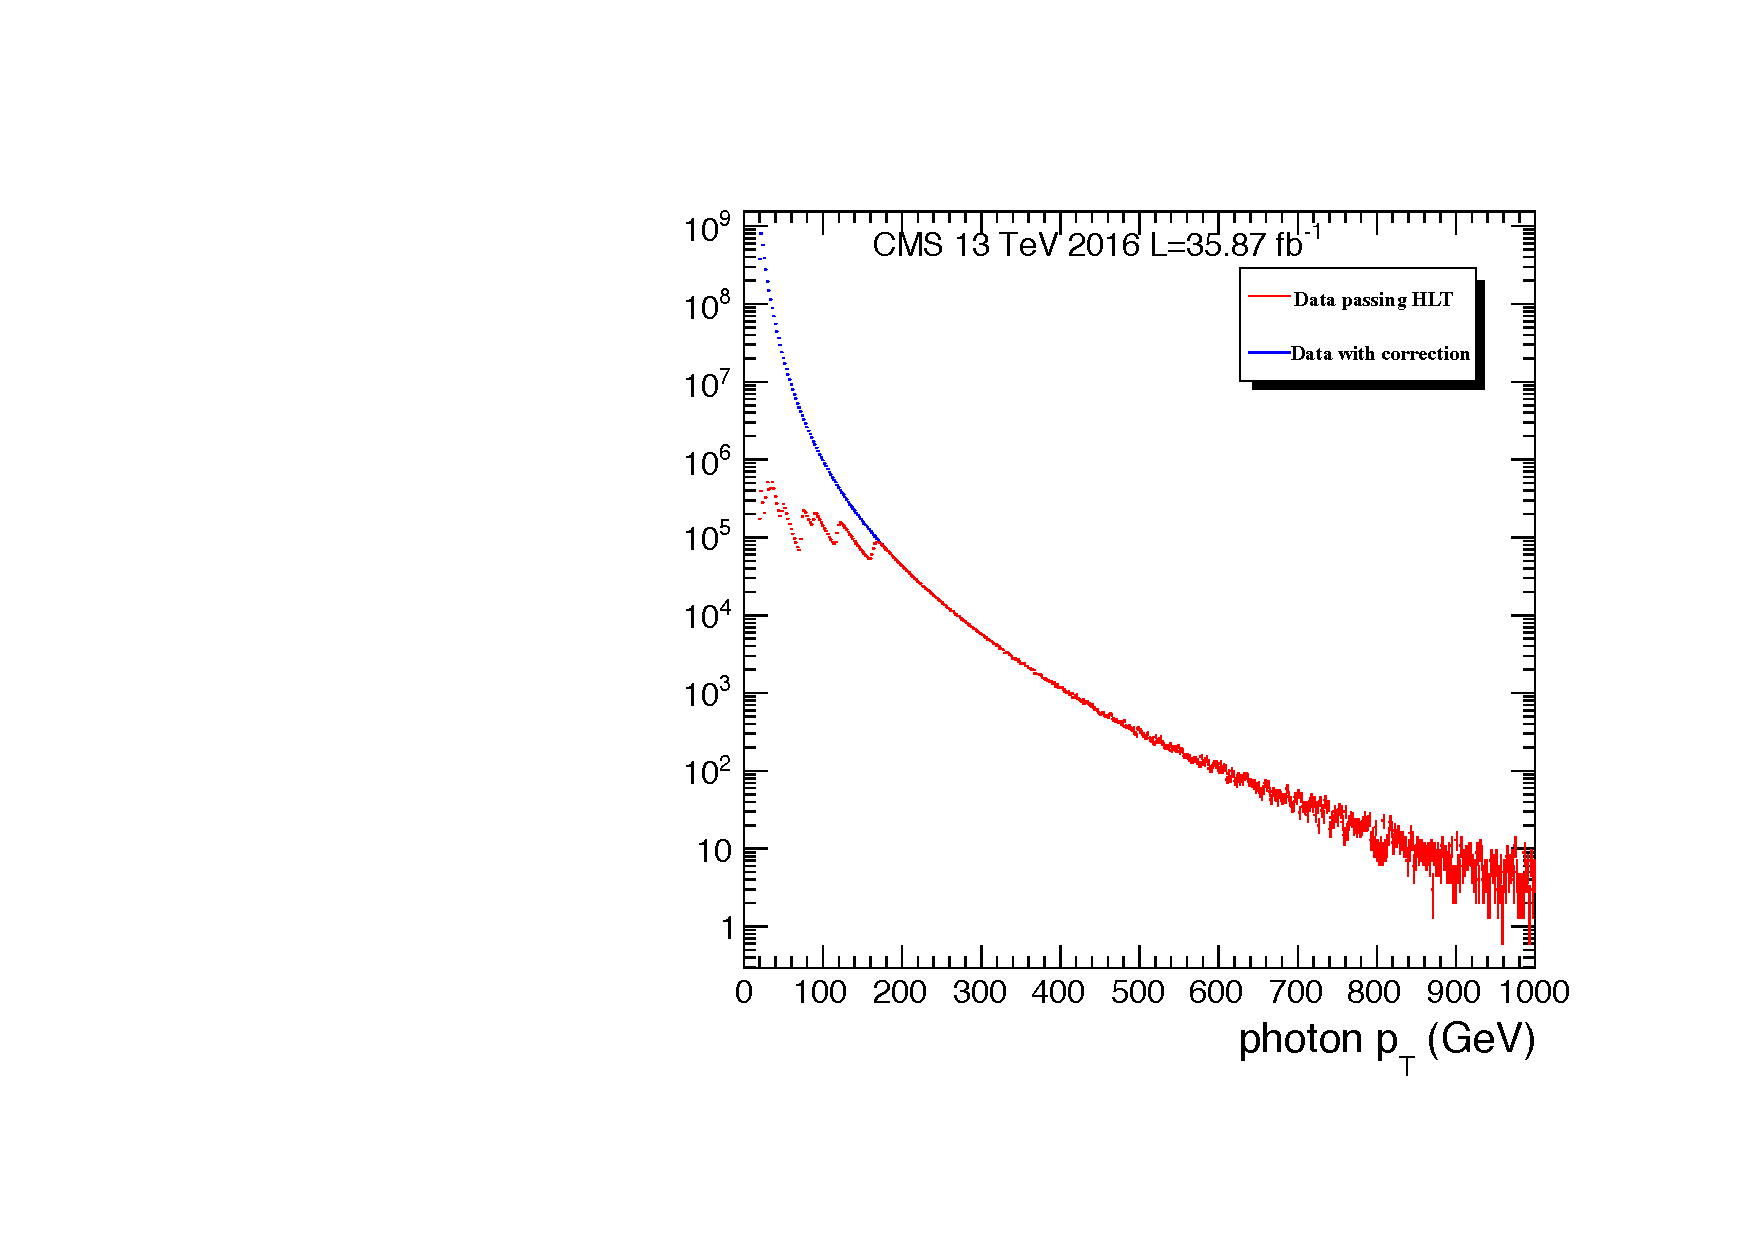
\includegraphics[width=0.86\linewidth]{figures/bg_photonHLT_reweight.pdf}
\caption{Photon $p_T$ distributions with and without the HLT prescale correction. }
\label{fig:photon_pt_prescale}
\end{center}
\end{figure}

\subsection{Physical ${p_{T}}^{miss}$ Subtraction}\label{sec:bg_gjetphysmet}
Like the Zjets process,  ${p_{T}}^{miss}$ in the process of $\gamma$jets are completely instrumental. However, processes like $W\gamma\rightarrow\ell\nu\gamma$ with physical ${p_{T}}^{miss}$ can also end in the SinglePhone dataset. To model the kinematics of the $\gamma$jets process better, events with physical ${p_{T}}^{miss}$ are subtracted from the SinglePhoton dataset using MC. MC samples shown in Table~\ref{tab:bg_photonMC} are used to describe the single photon dataset. Figures~\ref{fig:pho_met} and \ref{fig:pho_metpara} show the comparisons of the SinglePhoton data and MC for 2016 full dataset. The same set of SinglePhoton HLTs listed in Section~\ref{sec:bg_gjetHLT} has been applied on the MC samples, and the HLT prescale corrections are applies too. The discrepancy in the trigger efficiencies between MC and data is evaluated and addressed by the HLT efficiency corrections on the MC samples.

\begin{table}[htbh]
  \begin{center}
\begin{footnotesize}
    \caption{
      MC samples and their cross-sections for describing photon data and for physical ${p_{T}}^{miss}$ subtraction, Summer16 miniAODv2.
      \label{tab:bg_photonMC}}
    \begin{tabular}{l l}
      \hline
      MC Dataset & $\sigma [pb]$\\
      \hline\hline
  {\bf Instrumental ${p_{T}}^{miss}$ } & \\ \hline
       GJets\_HT-*To*\_TuneCUETP8M1\_13TeV-madgraphMLM-pythia8 & 32701  (LO) \\
       QCD\_Pt-*to*\_EMEnriched\_TuneCUETP8M1\_13TeV\_pythia8 & $1.86049\times 10^{7}$ (LO) \\
      \hline
      \hline
     {\bf Physical ${p_{T}}^{miss}$ } &\\ \hline
       DYJetsToLL\_M-50\_TuneCUETP8M1\_13TeV-amcatnloFXFX-pythia8 & $5765.4$  (NNLO)\\
       ZJetsToNuNu\_HT-*To*\_13TeV-madgraph & $457.081$  (NLO)\\
       WJetsToLNu\_HT-*To*\_TuneCUETP8M1\_13TeV-madgraphMLM-pythia8    & $2144.75$ (NLO) \\
       ZNuNuGJets\_MonoPhoton\_PtG-130\_TuneCUETP8M1\_13TeV-madgrap & $0.183\times1.43$ \\
       ZNuNuGJets\_MonoPhoton\_PtG-40to130\_TuneCUETP8M1\_13TeV-madgrap & $2.816\times1.43$ \\
       WGToLNuG\_TuneCUETP8M1\_13TeV-madgraphMLM-pythia8 & $585.8\times2.51$ \\
       TTGJets\_TuneCUETP8M1\_13TeV-amcatnloFXFX-madspin-pythia8 & 3.697 (NLO) \\
       ST\_t-channel\_top\_4f\_leptonDecays\_13TeV-powheg-pythia8\_TuneCUETP8M1 & 136.02 (NLO)\\
       ST\_t-channel\_antitop\_4f\_leptonDecays\_13TeV-powheg-pythia8\_TuneCUETP8M1 & 80.95 (NLO)\\
       ST\_tW\_top\_5f\_inclusiveDecays\_13TeV-powheg-pythia8\_TuneCUETP8M1 & 35.6  (NNLO)\\
       ST\_tW\_antitop\_5f\_inclusiveDecays\_13TeV-powheg-pythia8\_TuneCUETP8M1 & 35.6  (NNLO)\\
       TGJets\_TuneCUETP8M1\_13TeV\_amcatnlo\_madspin\_pythia8 & 2.967 (NLO)\\
      \hline\hline
    \end{tabular}
    \end{footnotesize}
  \end{center}
\end{table}


\begin{figure}[htbp!]
\centering
\includegraphics[width=0.48\linewidth, page=3]{figures/ReMiniAODSummer16HLT_FixXsec_SepProc_PhPtWt_tight_puWeightsummer16_unblind_log_.pdf}
\includegraphics[width=0.48\linewidth, page=5]{figures/ReMiniAODSummer16HLT_FixXsec_SepProc_PhPtWt_tight_puWeightsummer16_unblind_log_.pdf}
\caption{The photon ${p_T}$ (left) and $\eta$ (right) distributions and the MC sample description for the SinglePhoton dataset. }
\label{fig:pho_met}
\end{figure}

\begin{figure}[htbp!]
\centering
\includegraphics[width=0.48\linewidth, page=7]{figures/ReMiniAODSummer16HLT_FixXsec_SepProc_PhPtWt_tight_puWeightsummer16_unblind_log_.pdf}
\includegraphics[width=0.48\linewidth, page=8]{figures/ReMiniAODSummer16HLT_FixXsec_SepProc_PhPtWt_tight_puWeightsummer16_unblind_log_.pdf}
\caption{The photon ${p_{T}}^{miss}$ (left) and $\Delta \Phi (p_T ^\gamma ,p_T ^{miss})$ (right) distributions and the MC sample description for the SinglePhoton dataset. }
\label{fig:pho_metpara}
\end{figure}

\vspace{0.3cm}
The MC components with physical ${p_{T}}^{miss}$ in the final states, such as $Z\rightarrow\nu\nu$, $Z\gamma\rightarrow\nu\nu\gamma$, $W\gamma\rightarrow\ell\nu\gamma$, $W\rightarrow\ell\nu$, are subtracted from the SinglePhoton data, by merging these MC events into the photon data sample, with a weight of $-1$.

\subsection{${p_T}^{\gamma}$ to ${p_T}^Z$ Reweighting}\label{sec:bg_gjetpt}
The kinematic signature of $\gamma$jets events is expected to be similar to Zjets events, especially in the high energy region where the mass of Z bosons can be neglected. However, at lower energies the mass effects will alter the kinematics, and more importantly, the lepton selections applied in the Z boson reconstruction have different efficienies compared to that for the photon reconstruction. To address this issue, the photon $p_T$ distribution is reweighted to match that of the Z $p_T$. 

\vspace{0.3cm}
As there is no easy way to extract clean Z boson $p_T$ spectrum from the data with no background processes. The $p_T$ spectrum of the Z bosons is obtained from the MC sample DYJetsToLL\_M-50\_TuneCUETP8M1\_13TeV-amcatnloFXFX-pythia8, with inclusive cross-section of 5765.4 pb ($\pm 1.7\%$ PDF uncertainty) calculated at NNLO from FEWZ 3.1~\cite{bg_fewz}, and differential cross-section reweighted to the Zjets differential cross-section measured from the 2015 CMS data~\cite{bg_2015zjetxsec} on the generator level. The standard preselection is applied to the MC samples, with all efficiency reweightings applied. Figure~\ref{fig:photon_pt_weight_el} and \ref{fig:photon_pt_weight_mu} shows the photon $p_T$ reweighting function for electron channel and muon channel separately. 

\begin{figure}[htbp]
\centering
  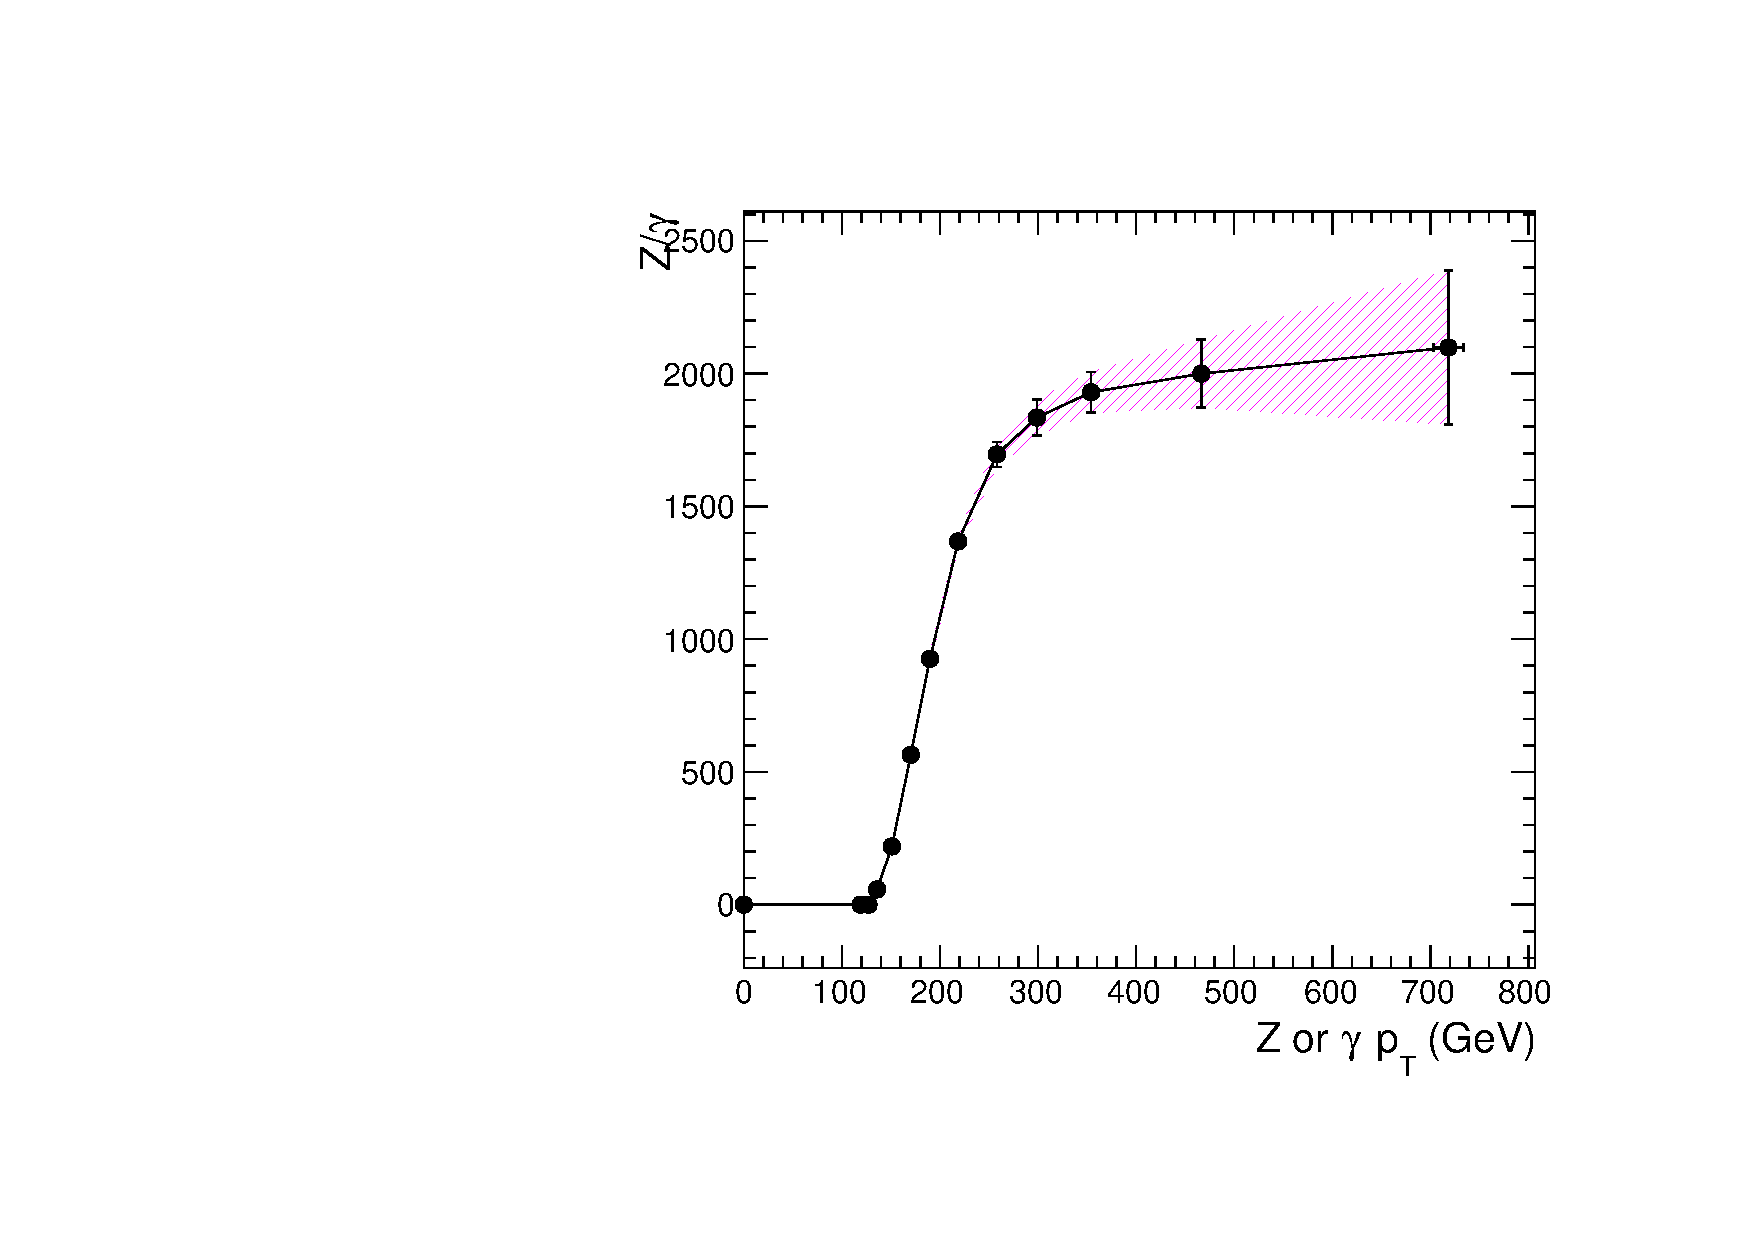
\includegraphics[width=0.9\linewidth]{figures/study_gjets_data_allcorV2_modify_el.pdf}
  \caption{Photon $p_T$ reweighting function for the electron channel.
 The uncertainty bands includes uncertainties from 2015 CMS Zjets differential cross-section measurements, the statistical uncertainty from Zjets MC sample and $\gamma$jets data sample, and the lepton trigger, ID, ISO efficiency scale factors.}
  \label{fig:photon_pt_weight_el}
\end{figure}

\begin{figure}[htbp]
\centering
  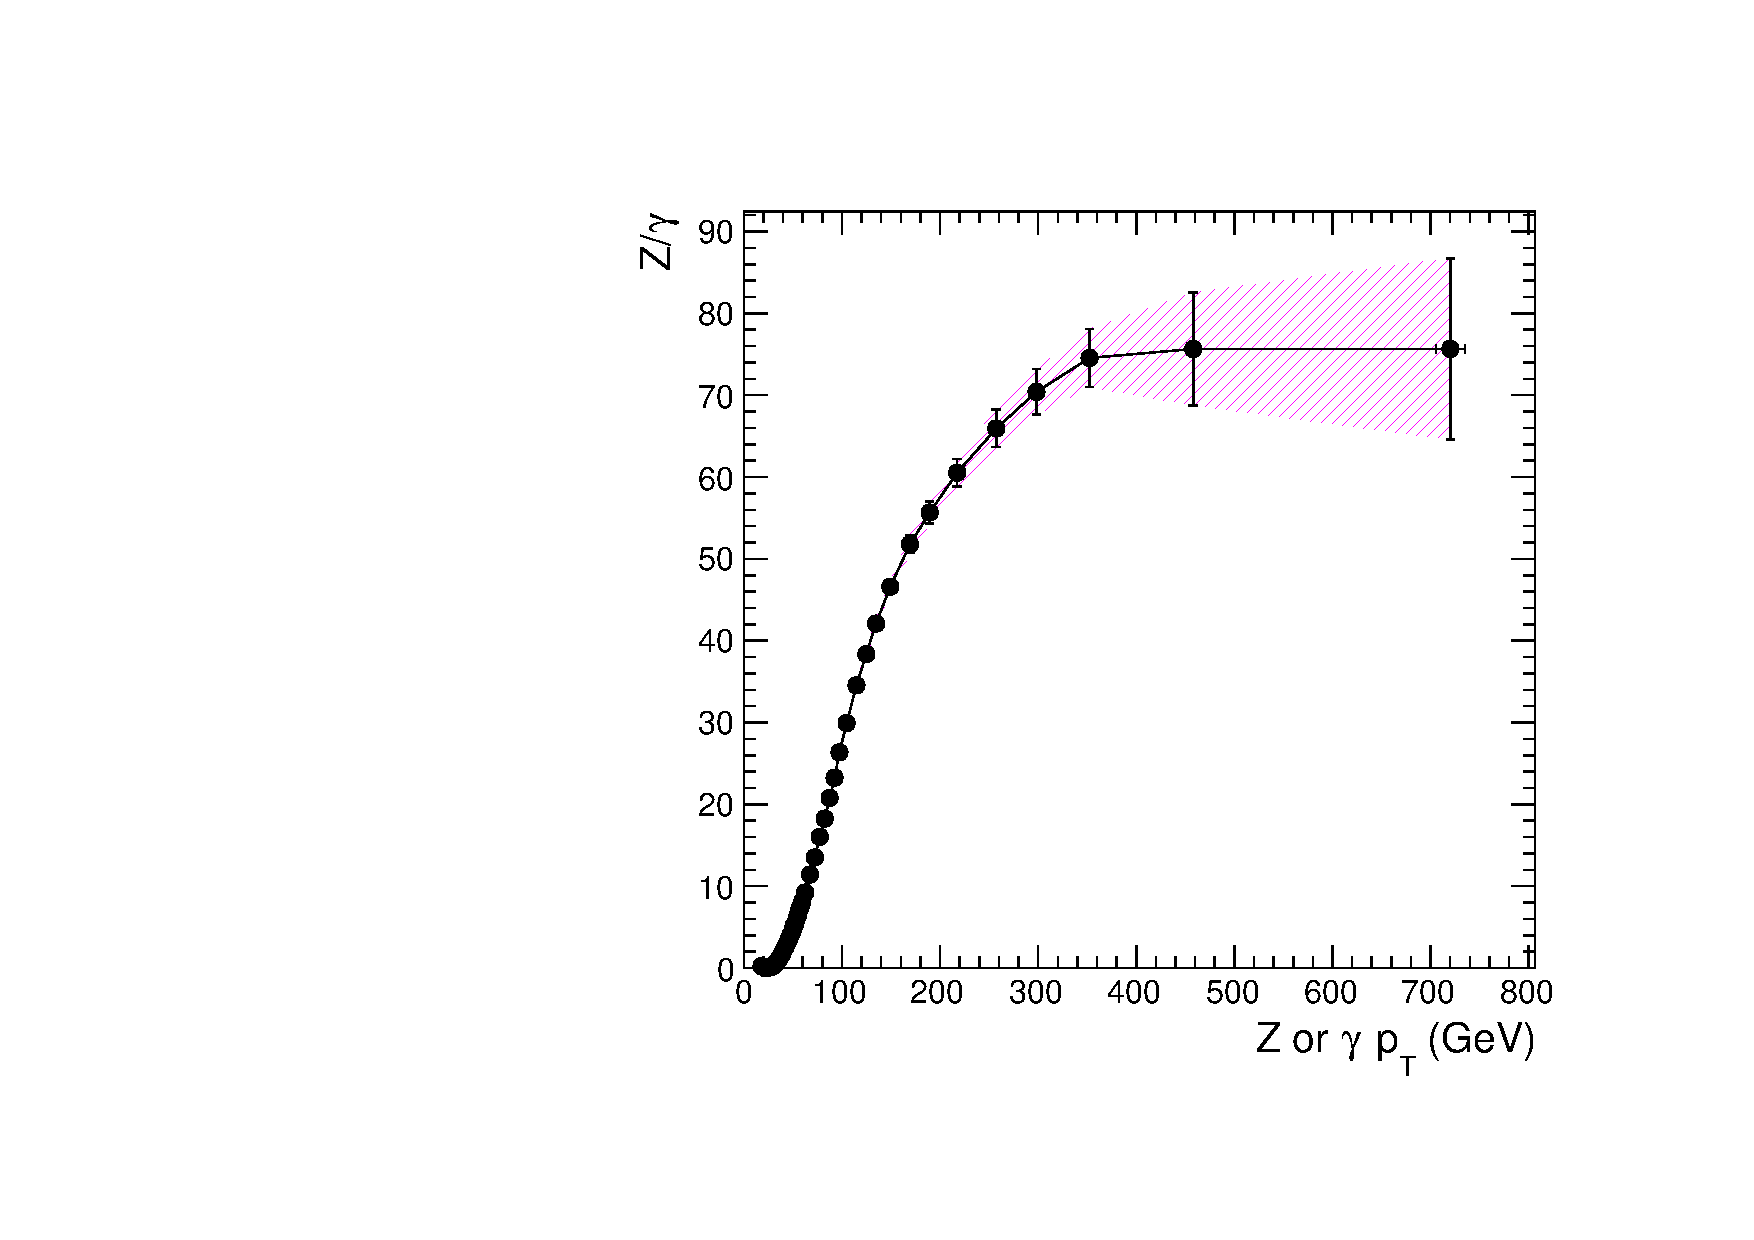
\includegraphics[width=0.9\linewidth]{figures/study_gjets_data_allcorV2_modify_mu.pdf}
  \caption{Photon $p_T$ reweighting function for the muon channel.
 The uncertainty bands includes uncertainties from 2015 CMS Zjets differential cross-section measurements, the statistical uncertainty from Zjets MC sample and $\gamma$jets data sample, and the lepton trigger, ID, ISO efficiency scale factors.}
  \label{fig:photon_pt_weight_mu}
\end{figure}

\subsection{Photon Mass Generation}\label{sec:gjetm}
The mass of the leptonic Z boson is used in the transverse mass calculation (Equation~\ref{eqn:intro_MT}, \ref{eqn:intro_MTalt}), and must be simulated in the $\gamma$jets events to model the $m_T$ in the Zjets background. This is done by assigning a random mass to the photon based on the Z boson mass distribution and parameterized as a function of Z boson $p_T$.

\vspace{0.3cm}
Figure~\ref{fig:mz_el_zjets_gjets} and \ref{fig:mz_mu_zjets_gjets}, compare the Z mass distributions of Zjets MC and the simulated Z mass for $\gamma$jets data events, for electron and muon channels separately.

\begin{figure}[htbp!]
\centering
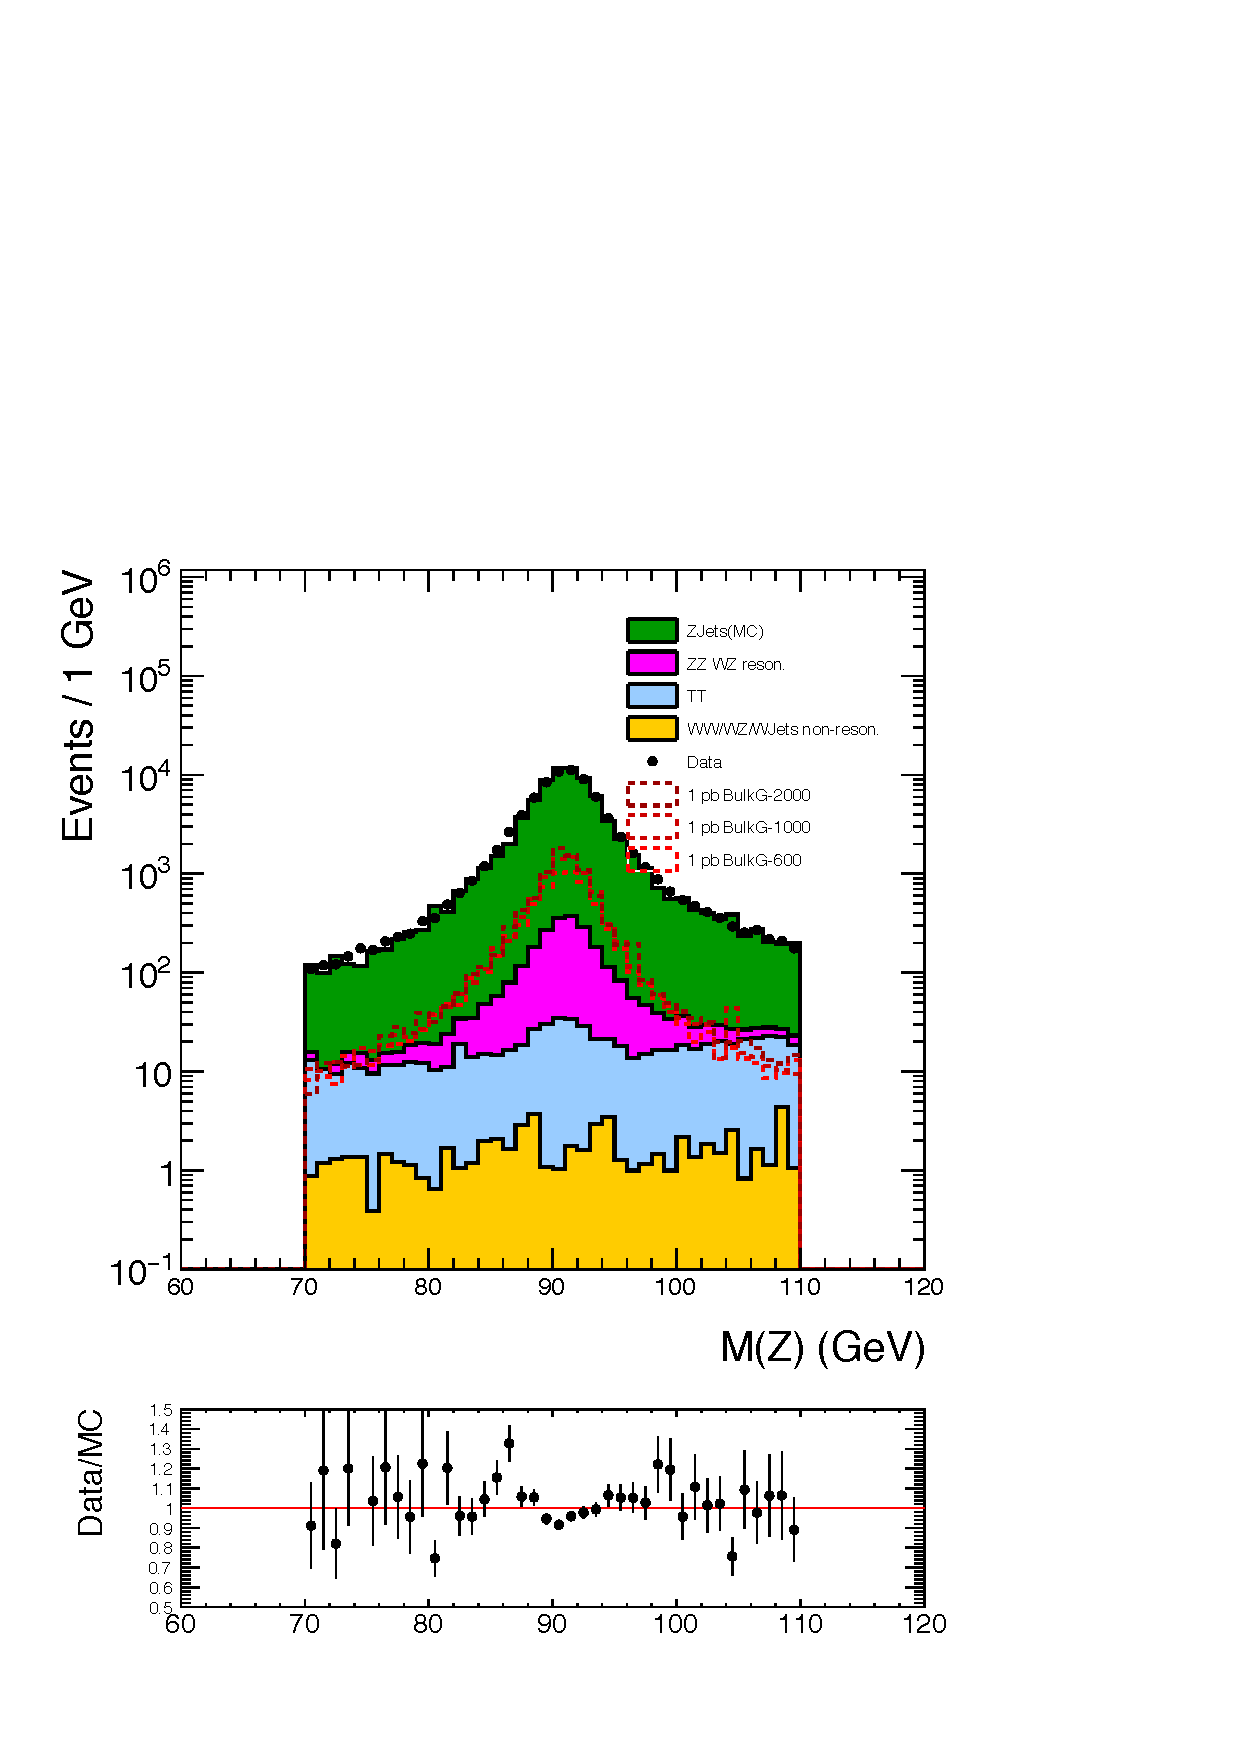
\includegraphics[width=0.46\linewidth]{figures/MC2_Rc36p46DtReCalib_RhoWt_GMCEtaWt_tightzpt50_puWeightmoriondMC_metfilter_el_log_1pb.pdf}
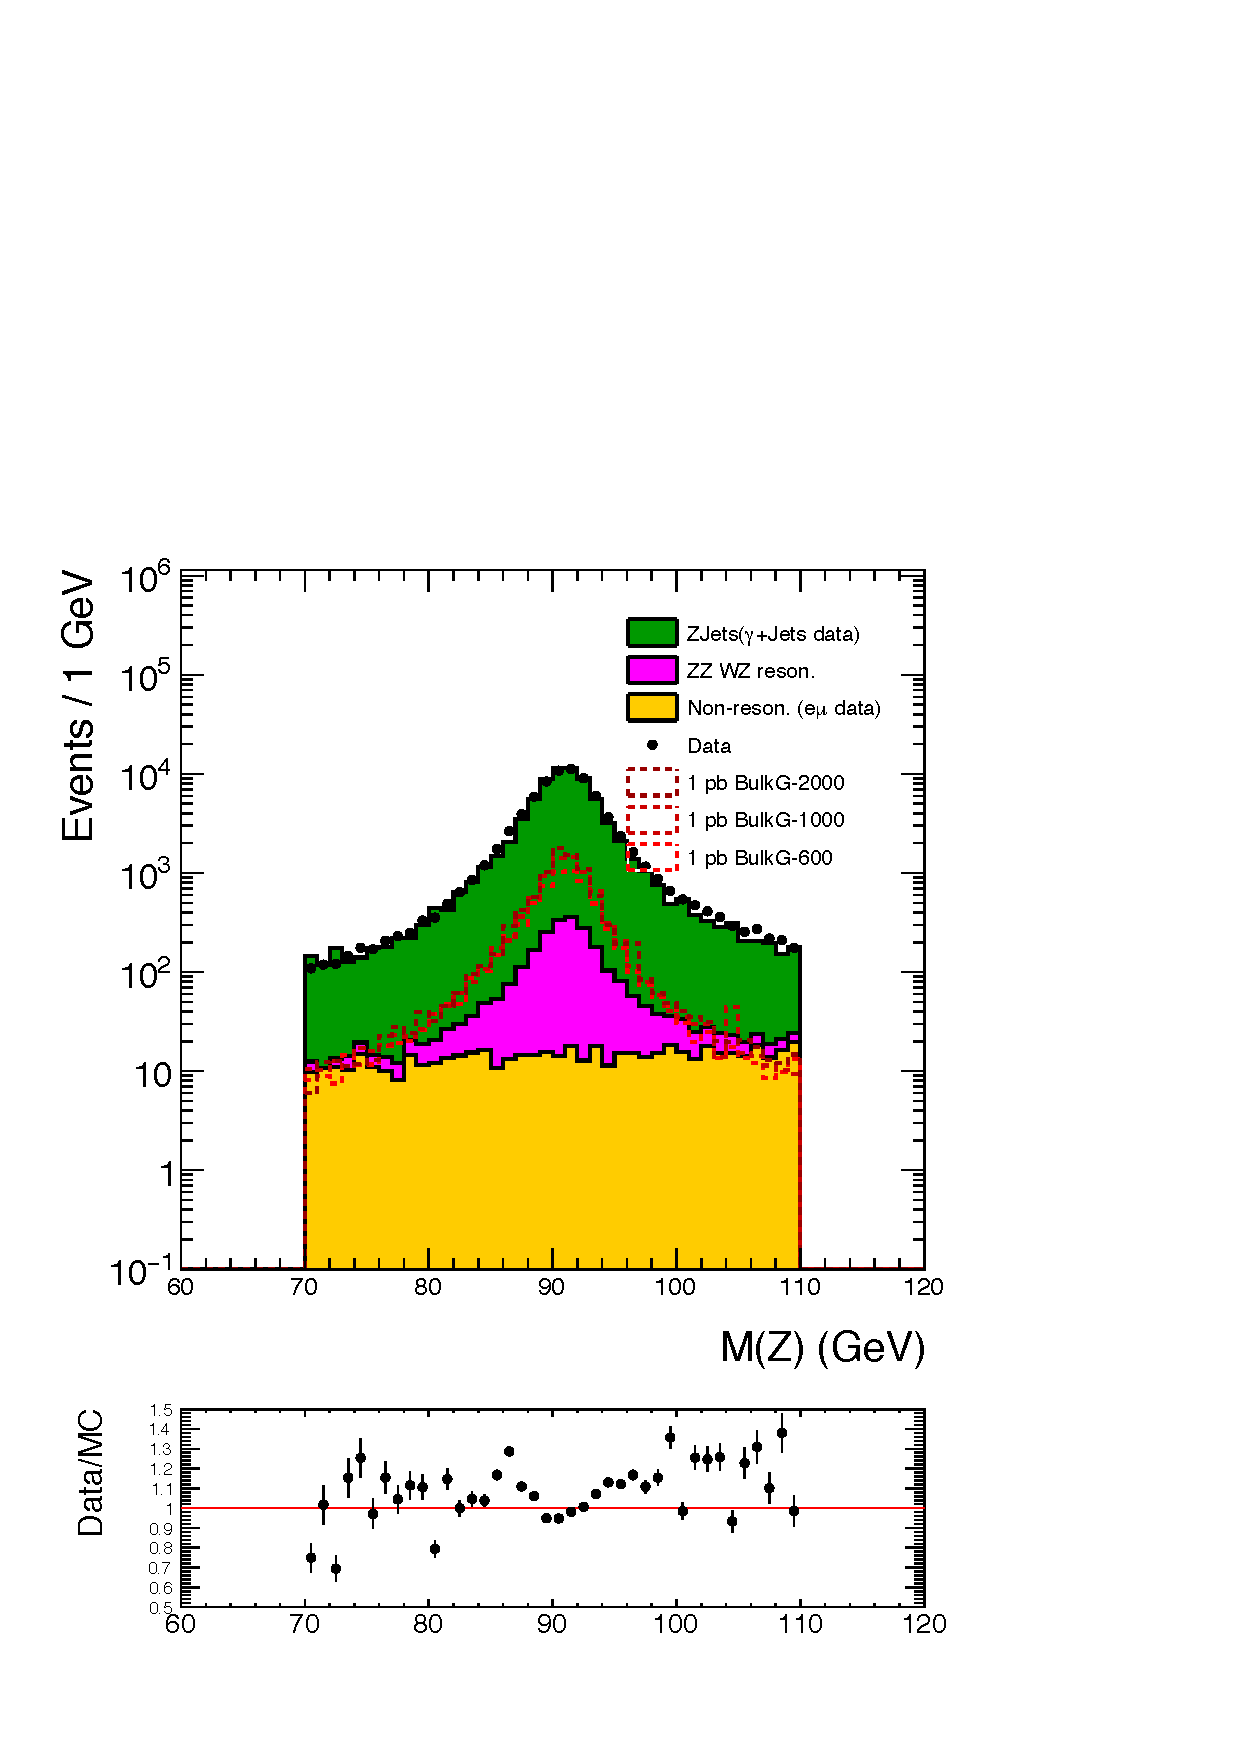
\includegraphics[width=0.46\linewidth]{figures/GJets2_BkgSub_Rc36p46DtReCalib_NonReso_RhoWt_GMCEtaWt_tightzpt50_puWeightmoriondMC_muoneg_gjet_metfilter_el_log_1pb.pdf}
\caption{Z mass distributions for electron channel, comparing Zjets MC (left) and the simulated Z mass for $\gamma$jets data events (right).}
\label{fig:mz_el_zjets_gjets}
\end{figure}

\begin{figure}[htbp!]
\centering
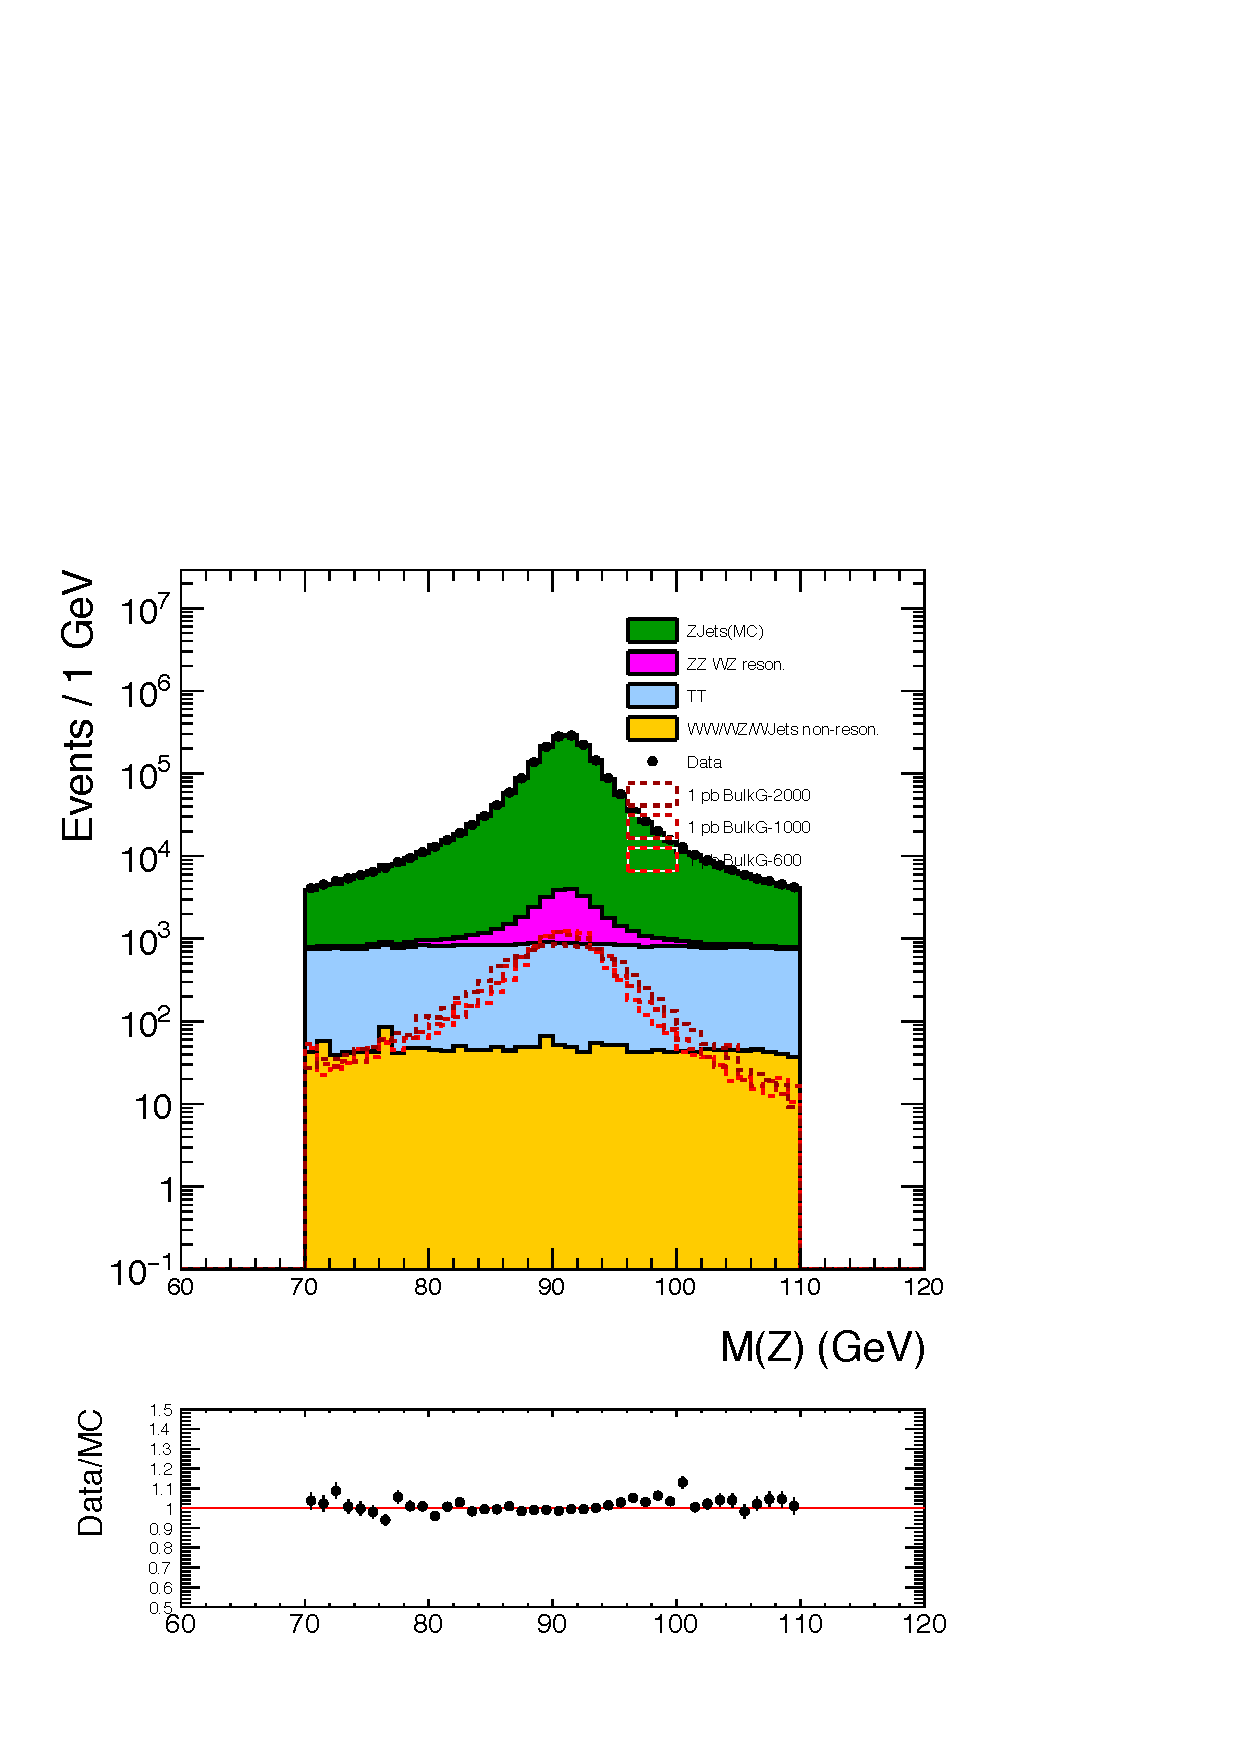
\includegraphics[width=0.46\linewidth]{figures/MC2_Rc36p46DtReCalib_RhoWt_GMCEtaWt_tightzpt50_puWeightmoriondMC_metfilter_mu_log_1pb.pdf}
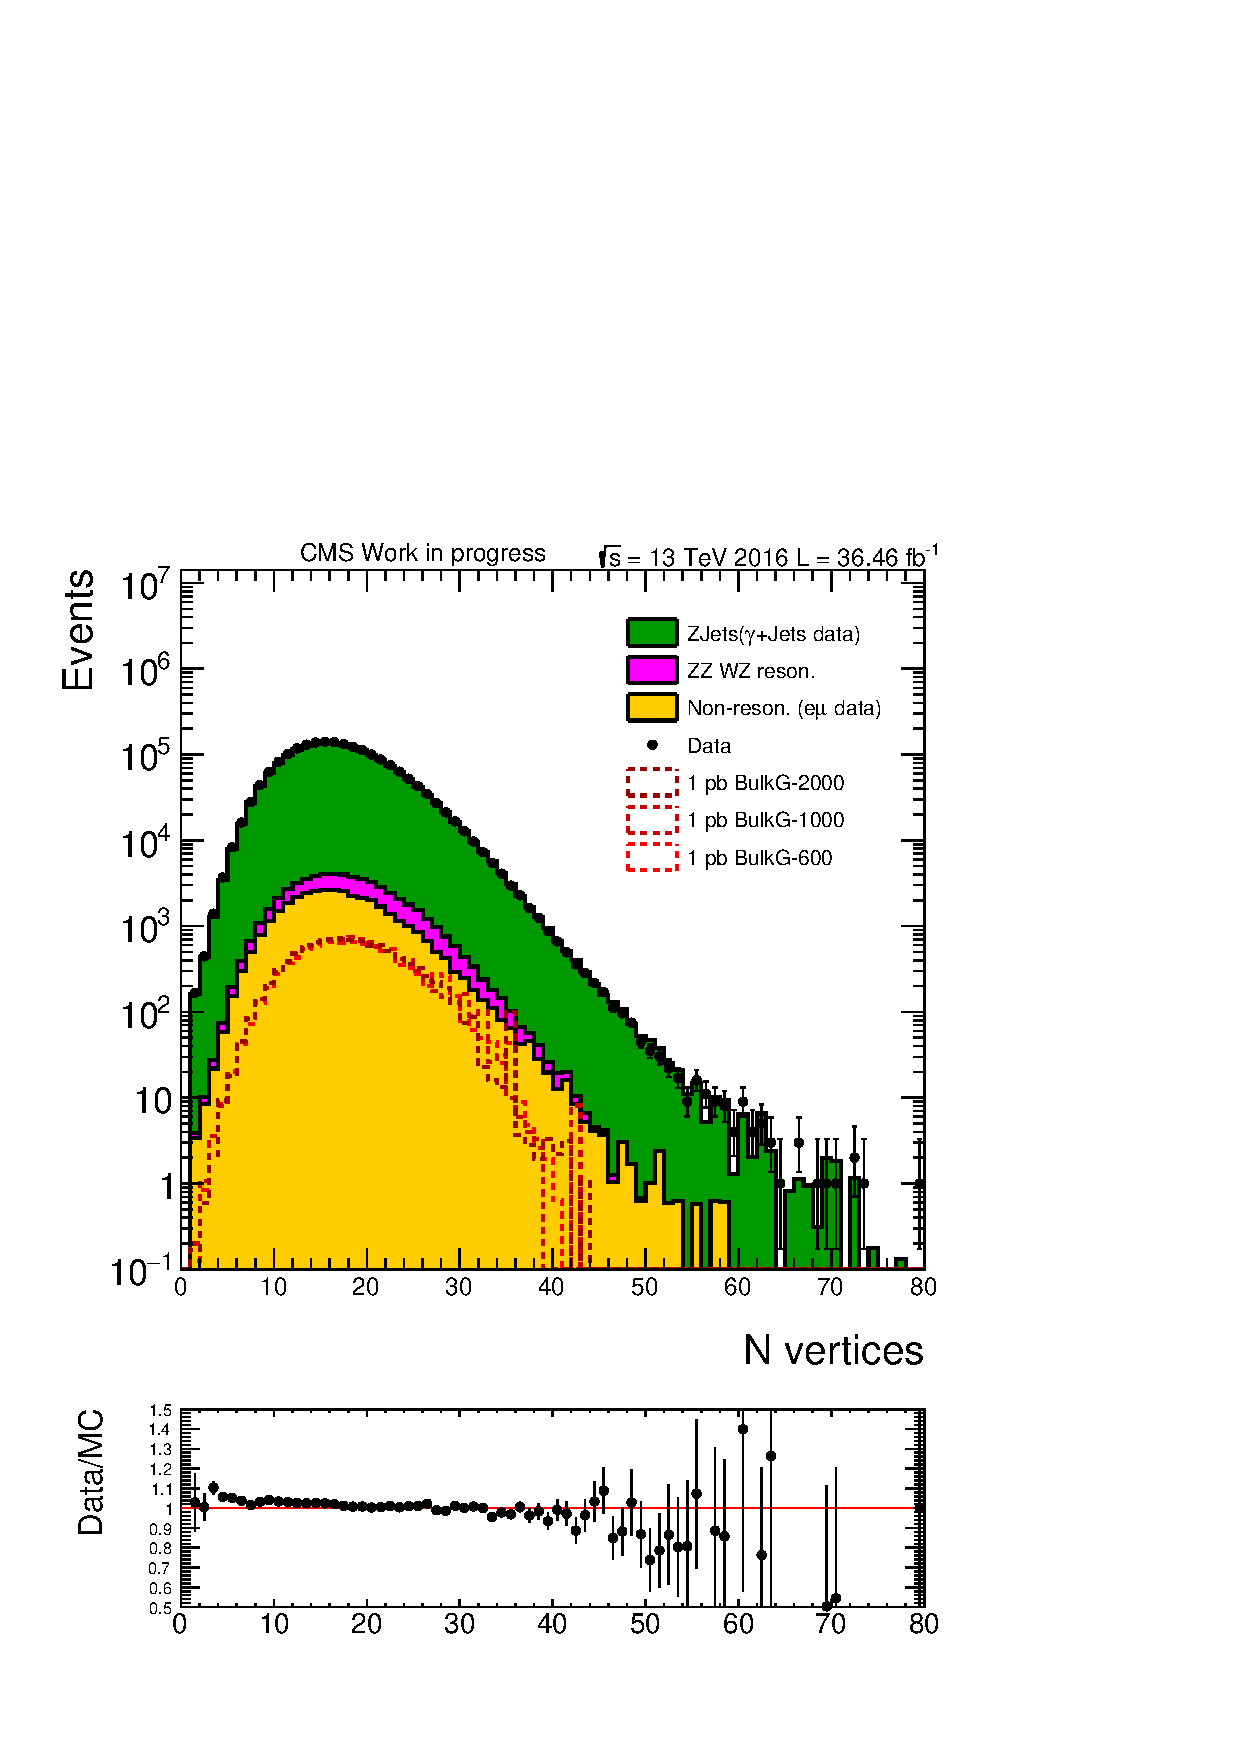
\includegraphics[width=0.46\linewidth]{figures/GJets2_BkgSub_Rc36p46DtReCalib_NonReso_RhoWt_GMCEtaWt_tightzpt50_puWeightmoriondMC_muoneg_gjet_metfilter_mu_log_1pb.pdf}
\caption{Z mass distributions for muon channel, comparing Zjets MC (left) and the simulated Z mass for $\gamma$jets data events (right).}
\label{fig:mz_mu_zjets_gjets}
\end{figure}

\subsection{${p_{T}}^{miss}$ Hadronic Recoil Tuning}\label{sec:gjetmet}
The Zjets process consists of a Z boson to a lepton pair and a hadronic recoil that balancing the Z boson $p_T$ in the transverse plain. As a result, in theory the ${p_{T}}^{miss}$ should be 0. However, due to the limitation on the detector resolutions of leptons and jets, the ${p_{T}}^{miss}$ in Zjets process exists and is purely instrumental. The ${p_{T}}^{miss}$ The energy resolutions of leptons, jets, photons are potentially different between $\gamma$jets data and Zjets data, and those differences may introduce difference in the resolution and scale of reconstructed ${p_{T}}^{miss}$.

\vspace{0.3cm}
A single-Gaussian based hadronic recoil fit is developed to tune the ${p_{T}}^{miss}$ of the $\gamma$jets data to match the ${p_{T}}^{miss}$ in the Zjets data. The general idea is to apply correction to the $\gamma$jets data to better discribe the ${p_{T}}^{miss}_\parallel$ and ${p_{T}}^{miss}_\perp$ distributions of the Zjets process, where ${p_{T}}^{miss}_\parallel$ refers to the projection of ${p_{T}}^{miss}$ in the direction of ${p}_{T}^{z(\gamma)}$ and ${p_{T}}^{miss}_\perp$ is the fraction perpendicular to ${p}_{T}^{z(\gamma)}$. 

\vspace{0.3cm}
The ${p_{T}}^{miss}_\parallel$ and ${p_{T}}^{miss}_\perp$ are fit with a Gaussian function in the region of [-50, 50] GeV. The Gaussian mean values and resolutions are parameterized as functions of the $p_T$ of Z boson and photon. Figure~\ref{fig:recoilfit_example_data} give some example plots showing the Gaussian fits for the $p_T$ bins 50-60 GeV for Zjets data, for muon channel and electron channel, for ${p_{T}}^{miss}_\parallel$ and ${p_{T}}^{miss}_\perp$, respectively.
\begin{figure}[htbp]
\begin{center}
\includegraphics[width=0.46\linewidth, page=21]{figures/SingleEMU_Run2016Full_03Feb2017_allcorV2_met_para_study_ZSelecLowLPt_mu.pdf}
\includegraphics[width=0.46\linewidth, page=56]{figures/SingleEMU_Run2016Full_03Feb2017_allcorV2_met_para_study_ZSelecLowLPt_mu.pdf}
\includegraphics[width=0.46\linewidth, page=21]{figures/SingleEMU_Run2016Full_03Feb2017_allcorV2_met_para_study_ZSelecLowLPt_el.pdf}
\includegraphics[width=0.46\linewidth, page=56]{figures/SingleEMU_Run2016Full_03Feb2017_allcorV2_met_para_study_ZSelecLowLPt_el.pdf}
\caption{Example plots for single Gaussian-based ${p_{T}}^{miss}$ hadronic recoil fit of selected Z $p_T$ bin for Zjets data, muon channel (upper), electron channel (lower),${p_{T}}^{miss}_\parallel$ (left), ${p_{T}}^{miss}_\perp$ (right).}
\label{fig:recoilfit_example_data}
\end{center}
\end{figure}


\vspace{0.3cm}
The comparison of the recoil fit results between Zjets data and $\gamma$jets data before correction are shown in 
Figure~\ref{fig:recoilfit_met_peak_reso_compare_data_gjets_mu}
and \ref{fig:recoilfit_met_peak_reso_compare_data_gjets_el}
for muon channel and electron channel respectively. 

\begin{figure}[htbp]
\begin{center}
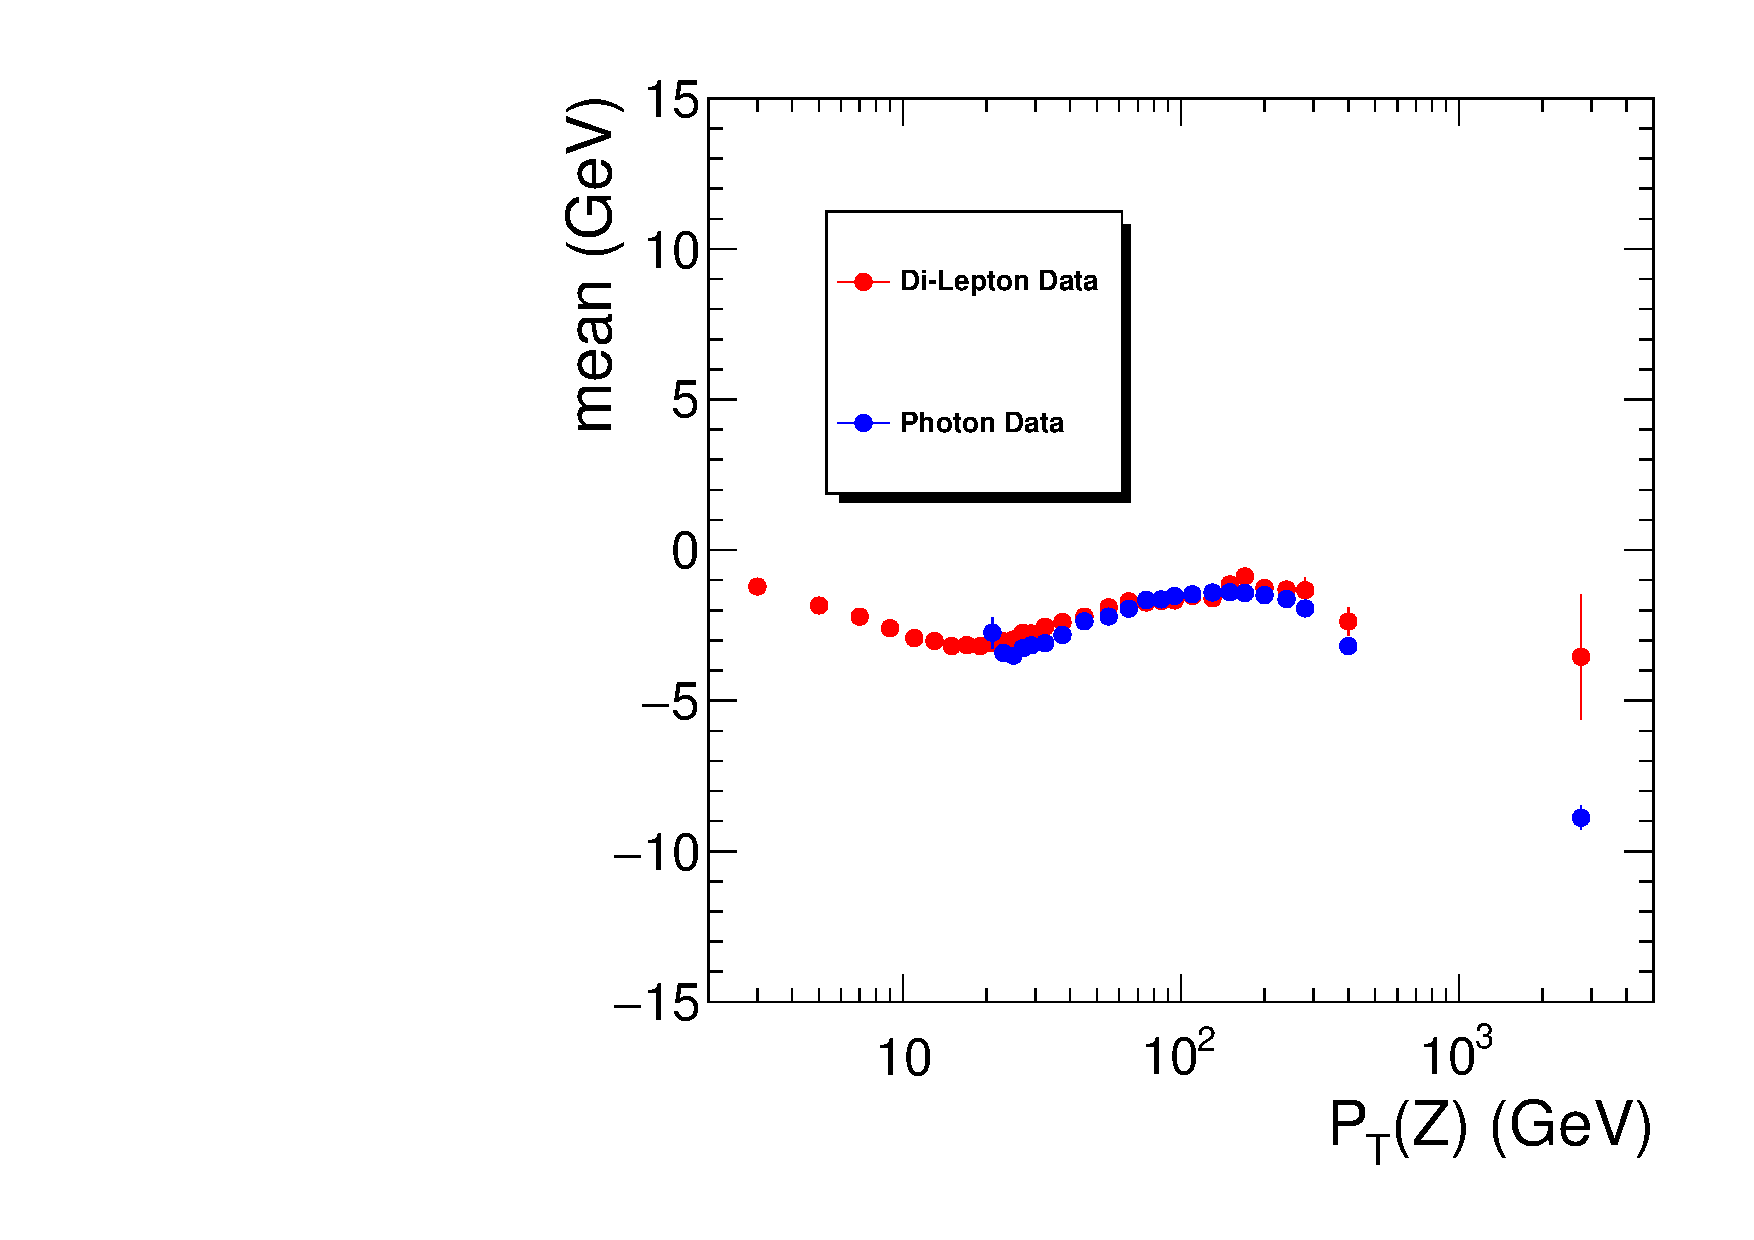
\includegraphics[width=0.46\linewidth, page=1]{figures/plots_SingleEMU_Run2016Full_03Feb2017_allcorV2_met_para_study_ZSelecLowLPt_mu_VS_SinglePhoton_Run2016Full_03Feb2017_allcorV2_NoRecoil_met_para_study_ZSelecLowLPt_mu.pdf}
\includegraphics[width=0.46\linewidth, page=5]{figures/plots_SingleEMU_Run2016Full_03Feb2017_allcorV2_met_para_study_ZSelecLowLPt_mu_VS_SinglePhoton_Run2016Full_03Feb2017_allcorV2_NoRecoil_met_para_study_ZSelecLowLPt_mu.pdf}
\includegraphics[width=0.46\linewidth, page=3]{figures/plots_SingleEMU_Run2016Full_03Feb2017_allcorV2_met_para_study_ZSelecLowLPt_mu_VS_SinglePhoton_Run2016Full_03Feb2017_allcorV2_NoRecoil_met_para_study_ZSelecLowLPt_mu.pdf}
\includegraphics[width=0.46\linewidth, page=7]{figures/plots_SingleEMU_Run2016Full_03Feb2017_allcorV2_met_para_study_ZSelecLowLPt_mu_VS_SinglePhoton_Run2016Full_03Feb2017_allcorV2_NoRecoil_met_para_study_ZSelecLowLPt_mu.pdf}
\caption{Comparison of the recoil fitted peak positions and Gaussian resolutions for ${p_{T}}^{miss}_\parallel$ and ${p_{T}}^{miss}_\perp$ between di-lepton data and $\gamma$jets data for the muon channel. Upper two for 
${p_{T}}^{miss}_\parallel$, bottom two for ${p_{T}}^{miss}_\perp$.}
\label{fig:recoilfit_met_peak_reso_compare_data_gjets_mu}
\end{center}
\end{figure}

\begin{figure}[htbp]
\begin{center}
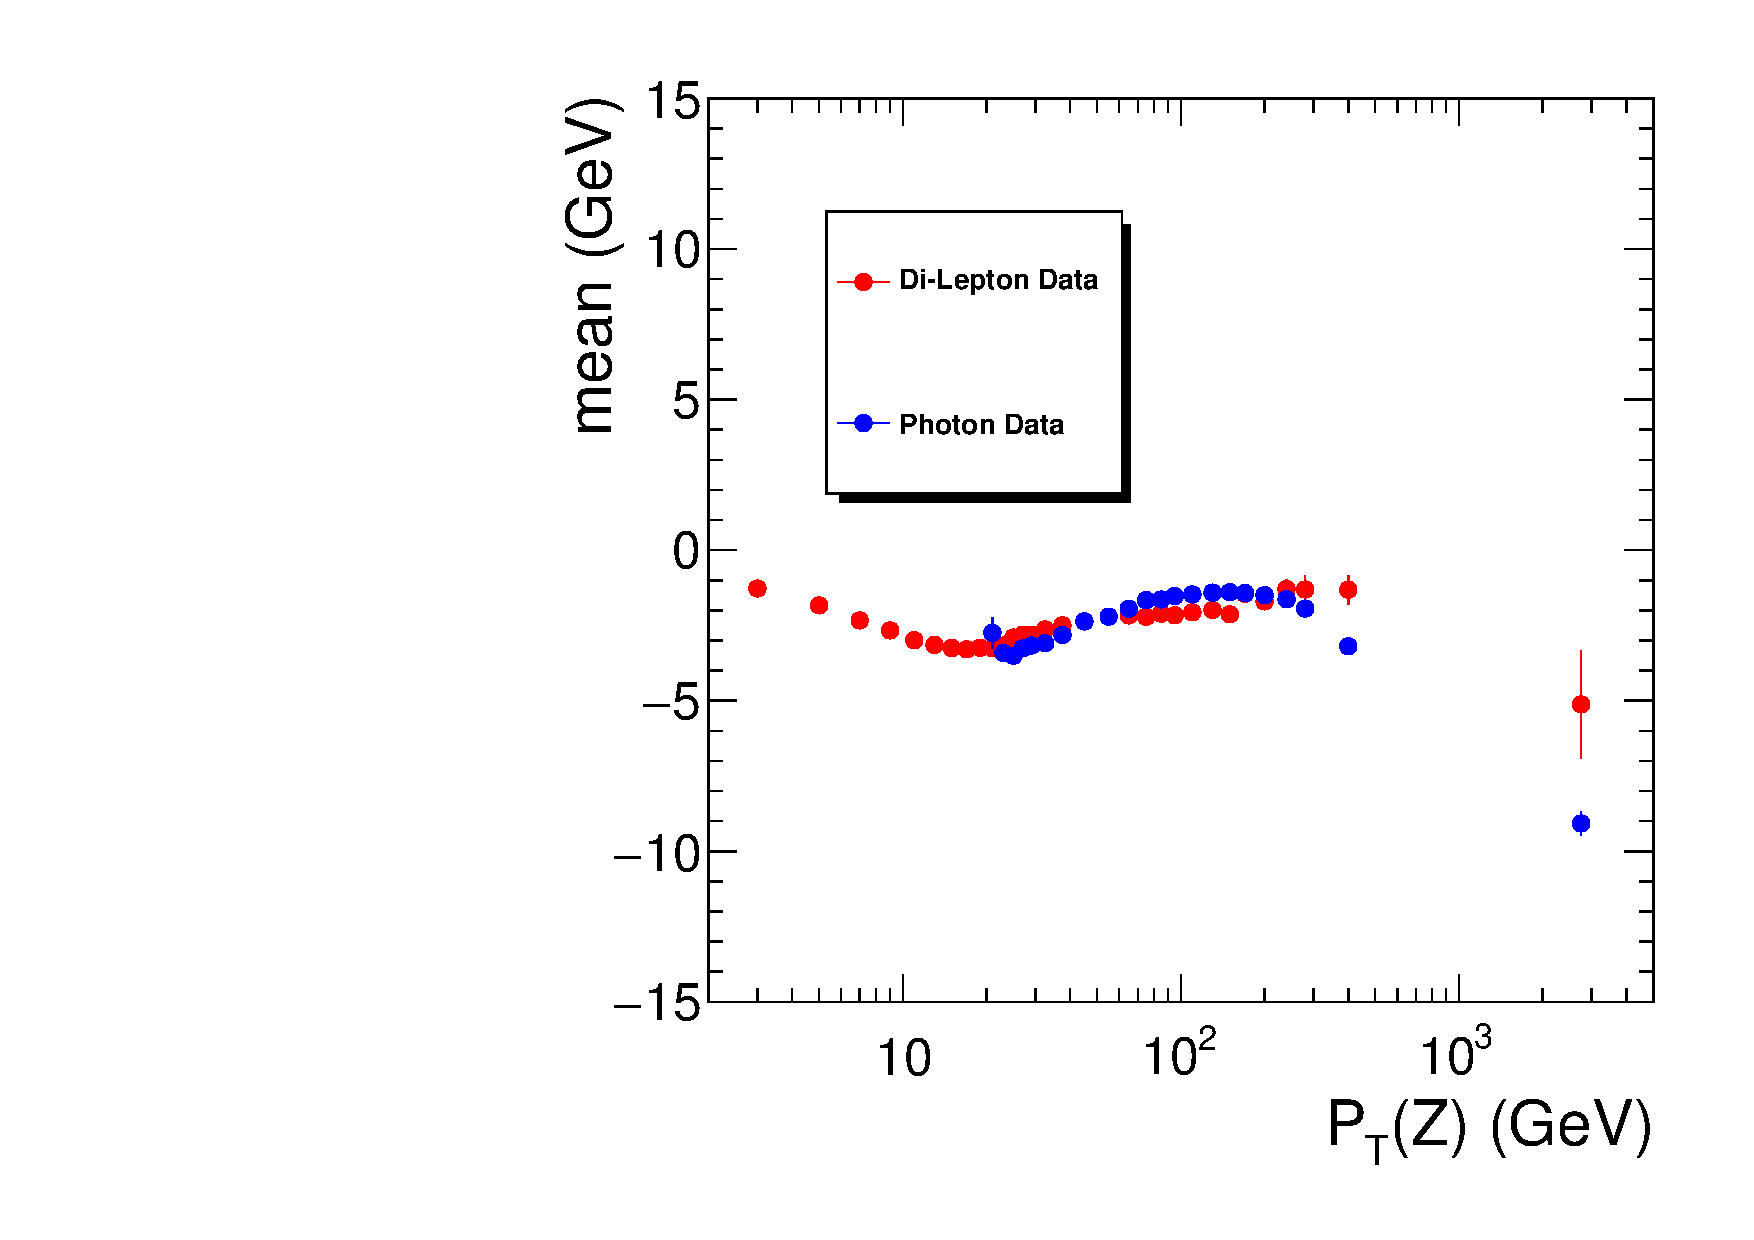
\includegraphics[width=0.46\linewidth, page=1]{figures/plots_SingleEMU_Run2016Full_03Feb2017_allcorV2_met_para_study_ZSelecLowLPt_el_VS_SinglePhoton_Run2016Full_03Feb2017_allcorV2_NoRecoil_met_para_study_ZSelecLowLPt_el.pdf}
\includegraphics[width=0.46\linewidth, page=5]{figures/plots_SingleEMU_Run2016Full_03Feb2017_allcorV2_met_para_study_ZSelecLowLPt_el_VS_SinglePhoton_Run2016Full_03Feb2017_allcorV2_NoRecoil_met_para_study_ZSelecLowLPt_el.pdf}
\includegraphics[width=0.46\linewidth, page=3]{figures/plots_SingleEMU_Run2016Full_03Feb2017_allcorV2_met_para_study_ZSelecLowLPt_el_VS_SinglePhoton_Run2016Full_03Feb2017_allcorV2_NoRecoil_met_para_study_ZSelecLowLPt_el.pdf}
\includegraphics[width=0.46\linewidth, page=7]{figures/plots_SingleEMU_Run2016Full_03Feb2017_allcorV2_met_para_study_ZSelecLowLPt_el_VS_SinglePhoton_Run2016Full_03Feb2017_allcorV2_NoRecoil_met_para_study_ZSelecLowLPt_el.pdf}
\caption{Comparison of the recoil fitted peak positions and Gaussian resolutions for ${p_{T}}^{miss}_\parallel$ and ${p_{T}}^{miss}_\perp$ between di-lepton data and $\gamma$jets data for the electron channel. Upper two for 
${p_{T}}^{miss}_\parallel$, bottom two for ${p_{T}}^{miss}_\perp$.}
\label{fig:recoilfit_met_peak_reso_compare_data_gjets_el}
\end{center}
\end{figure}

The $\gamma$jets data ${p_{T}}^{miss}_\parallel$ peak and the resolution of ${p_{T}}^{miss}_\parallel$ and ${p_{T}}^{miss}_\perp$ are then corrected to match the Zjets data respectively for muon and electron channels based on Figure~\ref{fig:recoilfit_met_peak_reso_compare_data_gjets_mu} and \ref{fig:recoilfit_met_peak_reso_compare_data_gjets_el}. The correction for the photon data is done in the following way:
\begin{itemize}
\item Shift the ${p_{T}}^{miss}_\parallel$ peak positions of $\gamma$jets data to match that of the Zjets data;
\item Scale the ${p_{T}}^{miss}_\parallel$ and ${p_{T}}^{miss}_\perp$ resolution of $\gamma$jets data to match that of the Zjets data.
\end{itemize}

The peak position correction is only applied to ${p_{T}}^{miss}_\parallel$, as the ${p_{T}}^{miss}$ results from the instrumental imbalance between the Z boson and hadronic recoil, therefore the distribution of ${p_{T}}^{miss}_\parallel$ is more imbalanced while the peak position for ${p_{T}}^{miss}_\perp$ is expected to be 0.

\clearpage
\section{Non-resonant Background Modeling}
The non-resonant background contains mostly $t\bar{t}$ and WW events. A data driven method is used in the analysis to model the non-resonant background. The method is to use the $e\mu$ pairs to describe the non-resonant background in $\ell\ell$ (ee or $\mu \mu$) events, based on the fact that in $t\bar{t}$ and WW decays, $e\mu$ pairs have similar kinematic behavior and cross-section as the $\ell\ell$ (ee or $\mu \mu$) decay states.

\subsection{$e\mu$ Pair Selection}
The 35.8 fb$^{-1}$ 2016 MuonEG dataset is used for the $e\mu$ pair selection.  Events with one or more $e\mu$ pair are selected. If more than one $e\mu$ pair is present in an event, the pair with invariant mass closest to Z boson mass is selected (analogous to the data selection). Electrons are required to pass Loose ID with pfIso, and muons are required to pass High $p_T$ ID and tracker isolation. 

\vspace{0.3cm}
When the $e\mu$ sample is used as background in the electron channel the selections below are applied to match the requirements applied in data: 
\begin{itemize}
\item Leading lepton $p_{T}>120GeV$, $|\eta|<2.5$, 
\item Subleading lepton $p_{T}>35GeV$, $|\eta|<2.5$
\end{itemize}
When the sample is used in the muon channel the selections are:
\begin{itemize}
\item Leading lepton $p_{T}>55GeV$, $|\eta|<2.4$
\item Subleading lepton $p_{T}>20GeV$, $|\eta|<2.4$. 
\end{itemize}

\subsection{$e\mu$ Pair Event-based Reweighting}
Based on the assumption that electrons and muons have the same behavior in the non-resonant background, the distributions of kinematic variables for the electron and muon in the $e\mu$ pair are expected to be nearly identical. However, this symmetry is altered by triggers and reconstruction effects. Figure~\ref{fig:nonresmuelpt} shows the $p_T$ distribution of electron and muon, and their ratio in the MuonEG dataset.

\begin{figure}[htbp]
\begin{center}
\includegraphics[width=0.95\linewidth]{figures/nonresmuelpt.png}
\caption{electron and muon $p_T$ distribution (left) and ratio (right) in the $e\mu$ pair sample selected from MuonEG dataset.}
\label{fig:nonresmuelpt}
\end{center}
\end{figure}

\vspace{0.3cm}
The discrepancy between the $p_T$ distributions of electrons and muons can result from many factors, such as detector effects, triggers, identification criteria and isolation efficiencies. Event based weighting factors are calculated according to the ratio plot in Figure~\ref{fig:nonresmuelpt}(right). When modeling the electron channel, the correction factor of the event is set to be the ratio value corresponding to the muon $p_T$ in the $e\mu$ event. Reversly, when modeling the muon channel, the correction factor of the event is the inverse of the ratio value corresponding to the electron $p_T$.

\vspace{0.3cm}
Figure~\ref{fig:nonresmuelptel} shows the electron and muon $p_T$ distribution and ratio after the correction for the electron channel, and Figure~\ref{fig:nonresmuelptmu} is for the muon channel.

\begin{figure}[htbp]
\begin{center}
\includegraphics[width=0.95\linewidth]{figures/nonresmuelptel.png}
\caption{electron and muon $p_T$ distribution (left) and ratio (right) in the $e\mu$ pair sample (from MuonEG dataset) after the event based reweighting for the electron channel}
\label{fig:nonresmuelptel}
\end{center}
\end{figure}

\begin{figure}[htbp]
\begin{center}
\includegraphics[width=0.95\linewidth]{figures/nonresmuelptmu.png}
\caption{electron and muon $p_T$ distribution (left) and ratio (right) in the $e\mu$ pair sample (from MuonEG dataset) after the event based reweighting for the muon channel}
\label{fig:nonresmuelptmu}
\end{center}
\end{figure}

\vspace{0.3cm}
The agreement between the $p_T$ distributions of electrons and muons are improved with the event based reweighting for both the electron channel and muon channel. In the electron channel, both leptons behave like the electron before weighting, and in the muon channel both leptons behave like the muon before weighting. This reweighting suppresses the systematic uncertainty caused by the performance discrepancy between electrons and muons due to detector and reconstruction effects. With the reweighting there is still a ~2\% of disagreement between the $p_T$ distributions of electrons and muons, and this is quoted as the systematic uncertainty of the method.

\subsection{HLT Efficiency Reweighting}
The effect of the HLT in our $\ell \ell$ data selection is calculated and applied in the $e\mu$ sample to simulate the single lepton HLT. With the event based reweighting described above, the electrons and muons in the $e\mu$ pair sample behave very similarly and can be treated as $\ell \ell$ pairs for the purpose of background studies. Both SingleElectron and SingleMuon trigger efficiency for data are calculated for each event in the $e\mu$ pair data, corresponding to the leading lepton's $p_T$ and $\eta$, regardless of whether the leading lepton is a muon or an electron. The trigger efficiency for data is described in Section~\ref{sec:bkg_trig}. The SingleElectron trigger efficiency is applied when the sample is used in the electron channel, similarly the SingleMuon trigger efficiency is applied when the sample is used in the muon channel. The uncertainty of the trigger efficiency is evaluated and quoted as the standard deviation of the efficiencies among all the selected events for each channel (see Table~\ref{tab:nonresuncert}).

\vspace{0.3cm}
When applying the SingleLepton trigger efficiency on the MuonEG dataset to emulate the data HLT, the MuonEG dataset is expected to have full acceptance in our preselection region. This explains why no HLT is required in the MuonEG data selection process. By not requiring any MuonEG HLT, events passing any MuonEG HLTs are accepted. Considering the high $p_T$ threshold in the lepton selection, the acceptance of the dataset is high enough and this effect can be ignored compared to the single lepton trigger efficiency uncertainty. In fact, the acceptance of the MuonEG dataset has negligible effect as long as it is consistent in our preselection region, and the $e\mu$ sample is rescaled as discussed below. To clarify, the $p_T$ thresholds of the MuonEG dataset do not affect our event selection. For the muon channel, we require a leading lepton $pt>60 GeV$, and subleading lepton $pt>20 GeV$. The electron channel has higher lepton $p_T$ selection. The MuonEG dataset contains non-prescaled triggers:
\begin{itemize}
\item \texttt{HLT\_Mu23\_TrkIsoVVL\_Ele12\_CaloIdL\_TrackIdL\_IsoVL(\_DZ)} 
\item \texttt{HLT\_Mu12\_TrkIsoVVL\_Ele23\_CaloIdL\_TrackIdL\_IsoVL(\_DZ)}
\end{itemize}
and these $p_T$ thresholds are much lower than our $p_T$ selection.

\subsection{$e\mu$ Events Rescaling}
To rescale the $e\mu$ samples to fit the nonresonant background and study the agreement of the background sample and data, a nonresonant control region is defined. The scale factor is calculated by equation~\ref{eq:nonresscale}.
\begin{equation} \label{eq:nonresscale}
  Scale  =  \frac{N_{data,ll}-N_{MC,reson}}{N_{data,e\mu}}
\end{equation}

The $N_{data,ll}$ is the number of data events in the control region; $N_{MC,reson}$ is the number of background Z events in the control region, including Zjets background and resonant background; the $N_{data,e\mu}$ is the number of $e\mu$ pair events in the control region. To define the control region, the main idea is to suppress the standard deviation of the calculated scale factor. The standard deviation is calculated based on equation~\ref{eq:nonresscale}, and given in equation~\ref{eq:nonresscaledev}.
\begin{equation} \label{eq:nonresscaledev}
  \sigma_{Scale}  = \sqrt{\frac{\sigma^{2}_{N_{data,ll}}+\sigma^{2}_{N_{MC,reson}}}{(N_{data,ll}-N_{MC,reson})^{2}}+\frac{\sigma^{2}_{N_{data,e\mu}}}{N^{2}_{data,e\mu}}}\times \frac{N_{data,ll}-N_{MC,reson}}{N_{data,e\mu}}
\end{equation}

Here the statistical uncertainty is considered for both MC and data, and the PDF uncertainty is considered for resonant MC (1.5\%).

\vspace{0.3cm}
To suppress scale deviation and resonant background in the CR, selections below are applied: 
\begin{enumerate}
\item Z mass veto: invariant mass $M<70GeV$ or $M>110GeV$; 
\item $p_{T}^{Z} > X GeV$;
\end{enumerate}

To determine the X value ($p_{T}^{Z}$ cut level), a scan over various X values is performed. The calculated scale factor and uncertainty vs X is shown in Table~\ref{tab:nonressfdev}. X=60 gives relatively small uncertainty, and is used to define the control region. The scale uncertainty corresponding to X=60 is also counted as the systematic uncertainty.

\begin{table}[htbp]
  \begin{center}
    \caption{
      scale and deviation vs X($p_{T}^{Z}$ cut value) scan result.      
      \label{tab:nonressfdev}}
    \begin{tabular}{c c c}
      \hline\hline
      X & electron channel scale & muon channel scale\\
      \hline
      0  & 0.3442$\pm$0.0140 & 0.8215$\pm$0.0519 \\
      10 & 0.3442$\pm$0.0140 & 0.7762$\pm$0.0388 \\
      20 & 0.3442$\pm$0.0140 & 0.7364$\pm$0.0290 \\
      30 & 0.3442$\pm$0.0140 & 0.7046$\pm$0.0238 \\
      40 & 0.3442$\pm$0.0140 & 0.6962$\pm$0.0202 \\
      50 & 0.3443$\pm$0.0140 & 0.6895$\pm$0.0182 \\
      60 & 0.3463$\pm$0.0140 & 0.6871$\pm$0.0171 \\
      70 & 0.3490$\pm$0.0142 & 0.6907$\pm$0.0167 \\
      80 & 0.3560$\pm$0.0146 & 0.6952$\pm$0.0170 \\
      90 & 0.3635$\pm$0.0156 & 0.7092$\pm$0.0182 \\
      100 & 0.3733$\pm$0.0169 & 0.7249$\pm$0.0205 \\
      110 & 0.3771$\pm$0.0186 & 0.7402$\pm$0.0234 \\
      \hline\hline
    \end{tabular}
  \end{center}
\end{table}

\vspace{0.3cm}
Electron channel plots in the control region are shown in Figure~\ref{fig:nonreselcr} and those for the muon channel are shown in the Figure~\ref{fig:nonresmucr}.

\begin{figure}[htbp]
\begin{center}
\includegraphics[width=0.39\linewidth, page=1]{figures/test_metzpt50_RhoWt_puWeight68075_metfilter_el_.pdf}
\includegraphics[width=0.39\linewidth, page=2]{figures/test_metzpt50_RhoWt_puWeight68075_metfilter_el_.pdf}
\includegraphics[width=0.39\linewidth, page=3]{figures/test_metzpt50_RhoWt_puWeight68075_metfilter_el_.pdf}
\includegraphics[width=0.39\linewidth, page=4]{figures/test_metzpt50_RhoWt_puWeight68075_metfilter_el_.pdf}
\caption{Data-driven non-resonant background in the control region, electron channel plots}
\label{fig:nonreselcr}
\end{center}
\end{figure}

\begin{figure}[htbp]
\begin{center}
\includegraphics[width=0.39\linewidth, page=1]{figures/test_metzpt50_RhoWt_puWeight68075_metfilter_mu_.pdf}
\includegraphics[width=0.39\linewidth, page=2]{figures/test_metzpt50_RhoWt_puWeight68075_metfilter_mu_.pdf}
\includegraphics[width=0.39\linewidth, page=3]{figures/test_metzpt50_RhoWt_puWeight68075_metfilter_mu_.pdf}
\includegraphics[width=0.39\linewidth, page=4]{figures/test_metzpt50_RhoWt_puWeight68075_metfilter_mu_.pdf}
\caption{Data-driven non-resonant background in the control region, muon channel plots}
\label{fig:nonresmucr}
\end{center}
\end{figure}

\vspace{0.3cm}
The control region plots show that the resonant background is heavily suppressed in the CR and data driven non-resonant background agrees well with the data. Also nonresonant $e\mu$ events should have similar cross section compared to those in $\ell\ell$ events, which means that the sum of the scale factors in the electron channel and the muon channel should be close to 1. From Table~\ref{tab:nonressfdev} we see that at X=60, the scale factor is 0.346 for the electron channel, and 0.687 for the muon channel, adding up to 1.033, which agrees with the prediction.

\subsection{Comparing to MC Modeling}
Figure~\ref{fig:nonreselzmasscr100} is a comparison of the nonresonant background modeled by the data-driven method and the $t\bar{t}+WW$ MC samples as a cross-check of the data-driven method, with $70GeV<M_{Z}<110GeV$, ${p_{T}}^{miss}>50GeV$ and $p_{T}^{Z}>100GeV$ (standard signal region selections in this analysis), for electron channel. Similarly Figure~\ref{fig:nonresmuzmasscr100} shows the result for the muon channel. The data-driven modeling method generally gives a very similar non-resonant background distribution as the MC. However, in the electron channel the yield of the data-driven method is slightly higher than the MC modeling.

\begin{figure}[htbp]
\begin{center}
\includegraphics[width=0.39\linewidth, page=1]{figures/test_zpt100_log_RhoWt_puWeight68075_metfilter_el_.pdf}
\includegraphics[width=0.39\linewidth, page=3]{figures/test_zpt100_log_RhoWt_puWeight68075_metfilter_el_.pdf}
\includegraphics[width=0.39\linewidth, page=6]{figures/test_zpt100_log_RhoWt_puWeight68075_metfilter_el_.pdf}
\includegraphics[width=0.39\linewidth, page=2]{figures/test_zpt100_log_RhoWt_puWeight68075_metfilter_el_.pdf}
\includegraphics[width=0.39\linewidth, page=5]{figures/test_zpt100_log_RhoWt_puWeight68075_metfilter_el_.pdf}
\includegraphics[width=0.39\linewidth, page=4]{figures/test_zpt100_log_RhoWt_puWeight68075_metfilter_el_.pdf}
\caption{Data-driven non-resonant background and MC non-resonant background comparison, with Z mass selection and $p_{T}^{Z}>100GeV, {p_{T}}^{miss}>50GeV$, electron channel plots}
\label{fig:nonreselzmasscr100}
\end{center}
\end{figure}

\begin{figure}[htbp]
\begin{center}
\includegraphics[width=0.39\linewidth, page=1]{figures/test_zpt100_log_RhoWt_puWeight68075_metfilter_mu_.pdf}
\includegraphics[width=0.39\linewidth, page=3]{figures/test_zpt100_log_RhoWt_puWeight68075_metfilter_mu_.pdf}
\includegraphics[width=0.39\linewidth, page=6]{figures/test_zpt100_log_RhoWt_puWeight68075_metfilter_mu_.pdf}
\includegraphics[width=0.39\linewidth, page=2]{figures/test_zpt100_log_RhoWt_puWeight68075_metfilter_mu_.pdf}
\includegraphics[width=0.39\linewidth, page=5]{figures/test_zpt100_log_RhoWt_puWeight68075_metfilter_mu_.pdf}
\includegraphics[width=0.39\linewidth, page=4]{figures/test_zpt100_log_RhoWt_puWeight68075_metfilter_mu_.pdf}
\caption{Data-driven non-resonant background and MC non-resonant background comparison, with Z mass selection and $p_{T}^{Z}>100GeV, {p_{T}}^{miss}>50GeV$,muon channel plots}
\label{fig:nonresmuzmasscr100}
\end{center}
\end{figure}

\vspace{0.3cm}
The yield discrepancy is evaluated and half of the discrepancy value is quoted as a systematic uncertainty (6.7\% for electron channel).

\subsection{Uncertainty Table}
In addition to the systematic uncertainty of this data-driven method discussed above, differences in acceptance are considered. All muons have $|\eta|<2.4$, while in the electron channel, each lepton from real non-resonant background can also have $|\eta|$ between 2.4 and 2.5, which differs from the $e\mu$ pair data-driven background. Fortunately, less than 0.1\% events with $p_{T}^{Z}>100GeV, {p_{T}}^{miss}>50GeV$ in the electron channel have an electron with $|\eta|$ between 2.4 and 2.5, which means that the effect can be neglected. 

\vspace{0.3cm}
Table~\ref{tab:nonresuncert} summarizes the uncertainties that have been evaluated for this data-driven nonresonant background modeling method.
\begin{table}[htbp]
\begin{small}
  \begin{center}
    \caption{
      data-driven nonresonant modeling method uncertainties
      \label{tab:nonresuncert}}
    \begin{tabular}{c|c c}
      \hline\hline
      Uncertainty & electron channel & muon channel \\
      \hline
      $e\mu$ pair reweighting & 2\% & 2\% \\
      Trigger efficiency & 6.0\% & 1.3\% \\
      Stat. uncert. of Data and MC, PDF/QCD uncert. of subtracted MCs  & 4.0\% & 2.4\% \\
      Data-driven vs. MC disagreement & 6.7\% & 0.1\% \\
      \hline
      Total  & 10.0\% & 3.4\% \\
      \hline\hline
    \end{tabular}
  \end{center}
\end{small}
\end{table}

\clearpage
\section{Resonant Background Modeling}
The resonant background in this analysis contains mainly SM $qq\rightarrow ZZ\rightarrow 2\ell 2\nu$ process, as well as WZ processes and ZZ processes with $\ell\ell$qq or 4$\ell$ final states. This component of the background is modeled by MC samples. For the $qq\rightarrow ZZ\rightarrow 2\ell 2\nu$ sample (ZZTo2L2Nu\_13TeV\_powheg\_pythia8), NNLO QCD~\cite{bg_nnloqcd} and NLO EW corrections~\cite{bg_nloqed1,bg_nloqed2} are applied.

\vspace{0.3cm}
The NNLO/NLO QCD correction is parametrized and applied as a function of $m_{ZZ}$ 
at generator level. 
The correction and the uncertainty band are shown on Figure~\ref{fig:qqzz_nnlo_qcd}.
The average NNLO/NLO QCD correction k-factor is 1.11 with an uncertainty of 3\%.
For generator level $m_{ZZ}$~$>$~500~GeV, the average k-factor and uncertainty are applied. 

\begin{figure}[htbp!]
\centering
  \includegraphics[width=0.48\linewidth]{figures/h_nnlo_to_nlo_vs_mzz.pdf}
  \caption{The NNLO/NLO QCD correction and error band as a function of generator level $m_{ZZ}$ for SM qqZZ process.}
  \label{fig:qqzz_nnlo_qcd}
\end{figure}

\vspace{0.3cm}
The NLO/LO EW correction is parametrized as a function of initial states quark flavors and event kinematic variables $\hat{s}$ and $\hat{t}$
in the center of mass frame at generator level. 
The variable $\hat{s}$ is the partonic center of mass energy, corresponding to $m_{ZZ}$,
and $\hat{t}$ is computed as
\begin{align*}
\hat{t} = \left(p^*_{q_1}-p^*_{Z_1}\right)^2 & = p_{q_1}^{*2} +
p_{Z_1}^{*2} - 2 p^*_{q_1} \cdot p^*_{Z_1} \\
& \simeq 0 + m_{Z}^{2} - 2 \left( \frac{\hat{s}}{4} -
\frac{\sqrt{\hat{s}}}{2} \cos{\theta} \sqrt{\frac{\hat{s}}{4} -
m_{Z}^{2}} \right) \\
& = m_{Z}^{2} - \frac{\hat{s}}{2} + \cos{\theta}
\sqrt{\frac{\hat{s}^2}{4} - m_{Z}^{2}\hat{s}},
\end{align*}
where $p^*_{q_1}$ is the four momentum of the first quark initiating the hard process and 
$p^*_{Z_1}$  is the four momentum of the first Z boson, and quark masses are neglected.
The angle $\theta$ is the angle between the Z boson and the direction of the
incident quarks in the center-of-mass frame of the two Z bosons. 
Considering the radiation of gluons emitted at small angles, the direction of the incident
quarks is approximately computed as 
\begin{equation*}
\cos{\theta} = \frac{\hat{\vec{p}}_{q_1b} -
\hat{\vec{p}}_{q_2b}}{\left|\left( \hat{\vec{p}}_{q_1b} -
\hat{\vec{p}}_{q_2b} \right)\right|} \cdot \hat{\vec{p}}_{Z_1b},
\end{equation*}
where $\hat{\vec{p}}_{q_i/Z_ib}$ represents the unitary direction vector of the
$i$th quark/$Z$ boson after the Lorentz boost. 

\vspace{0.3cm}
The average k-factor for NLO/LO EW correction is 0.95 with an uncertainty of 3~\%. 
The correction function and the uncertainty band is shown on Figure~\ref{fig:qqzz_nlo_ew}
as a function of generator level $m_{ZZ}$. 
The NLO/LO EW correction is only appropriate for on-shell Z with $m_{ZZ}>2 m_{Z}$. 

\begin{figure}[htbp!]
\centering
  \includegraphics[width=0.48\linewidth]{figures/ewkfactor.pdf}
  \caption{The NLO/LO EW correction and error band as a function of generator level $m_{ZZ}$ for SM qqZZ process.}
  \label{fig:qqzz_nlo_ew}
\end{figure}

\clearpage
\section{Preselection Plots}
Figures~\ref{fig:gjet_rho} to \ref{fig:gjet_metperp} show the data vs background distributions in the preselection region, with all the backgrounds modeled using the methods discussed above. 

\begin{figure}[htbp!]
\centering
\includegraphics[width=0.46\linewidth, page=1]{figures/ReMiniSummer16_DT_PhReMiniMCRcFixXsec_GMCPhPtWt_tightzpt50_puWeightsummer16_muoneg_gjet_metfilter_unblind_el_log_1pb.pdf}
\includegraphics[width=0.46\linewidth, page=1]{figures/ReMiniSummer16_DT_PhReMiniMCRcFixXsec_GMCPhPtWt_tightzpt50_puWeightsummer16_muoneg_gjet_metfilter_unblind_mu_log_1pb.pdf}
\caption{Vertex multiplicity distributions for electron (left) and muon (right) channels
comparing data and background.}
\label{fig:gjet_nvtx}
\end{figure}

\begin{figure}[htbp!]
\centering
\includegraphics[width=0.46\linewidth, page=2]{figures/ReMiniSummer16_DT_PhReMiniMCRcFixXsec_GMCPhPtWt_tightzpt50_puWeightsummer16_muoneg_gjet_metfilter_unblind_el_log_1pb.pdf}
\includegraphics[width=0.46\linewidth, page=2]{figures/ReMiniSummer16_DT_PhReMiniMCRcFixXsec_GMCPhPtWt_tightzpt50_puWeightsummer16_muoneg_gjet_metfilter_unblind_mu_log_1pb.pdf}
\caption{$\rho$ distributions for electron (left) and muon (right)
channels comparing data and background.}
\label{fig:gjet_rho}
\end{figure}

\begin{figure}[htbp!]
\centering
\includegraphics[width=0.46\linewidth,page=3]{figures/ReMiniSummer16_DT_PhReMiniMCRcFixXsec_GMCPhPtWt_tightzpt50_puWeightsummer16_muoneg_gjet_metfilter_unblind_el_log_1pb.pdf}
\includegraphics[width=0.46\linewidth,page=3]{figures/ReMiniSummer16_DT_PhReMiniMCRcFixXsec_GMCPhPtWt_tightzpt50_puWeightsummer16_muoneg_gjet_metfilter_unblind_mu_log_1pb.pdf}
\caption{$m_T$ distributions for electron (left) and muon (right) channels
comparing data and background,
wide mass window.}
\label{fig:gjet_mt_wide}
\end{figure}

\begin{figure}[htbp!]
\centering
\includegraphics[width=0.46\linewidth,page=5]{figures/ReMiniSummer16_DT_PhReMiniMCRcFixXsec_GMCPhPtWt_tightzpt50_puWeightsummer16_muoneg_gjet_metfilter_unblind_el_log_1pb.pdf}
\includegraphics[width=0.46\linewidth,page=5]{figures/ReMiniSummer16_DT_PhReMiniMCRcFixXsec_GMCPhPtWt_tightzpt50_puWeightsummer16_muoneg_gjet_metfilter_unblind_mu_log_1pb.pdf}
\caption{$m_T$ distributions for electron (left) and muon (right) channels
comparing data and background,
narrow mass window.}
\label{fig:gjet_mt_narrow}
\end{figure}

\begin{figure}[htbp!]
\centering
\includegraphics[width=0.46\linewidth,page=8]{figures/ReMiniSummer16_DT_PhReMiniMCRcFixXsec_GMCPhPtWt_tightzpt50_puWeightsummer16_muoneg_gjet_metfilter_unblind_el_log_1pb.pdf}
\includegraphics[width=0.46\linewidth,page=8]{figures/ReMiniSummer16_DT_PhReMiniMCRcFixXsec_GMCPhPtWt_tightzpt50_puWeightsummer16_muoneg_gjet_metfilter_unblind_mu_log_1pb.pdf}
\caption{Z mass ($m_{\ell\ell}$) distributions for electron (left) and muon (right) channels
comparing data and background.}
\label{fig:gjet_mz}
\end{figure}

\begin{figure}[htbp!]
\centering
\includegraphics[width=0.46\linewidth,page=9]{figures/ReMiniSummer16_DT_PhReMiniMCRcFixXsec_GMCPhPtWt_tightzpt50_puWeightsummer16_muoneg_gjet_metfilter_unblind_el_log_1pb.pdf}
\includegraphics[width=0.46\linewidth,page=9]{figures/ReMiniSummer16_DT_PhReMiniMCRcFixXsec_GMCPhPtWt_tightzpt50_puWeightsummer16_muoneg_gjet_metfilter_unblind_mu_log_1pb.pdf}
\caption{${p_T}^Z$ distributions for electron (left) and muon (right) channels
comparing data and background,
wide binning.}
\label{fig:gjet_zpt_wide}
\end{figure}

\begin{figure}[htbp!]
\centering
\includegraphics[width=0.46\linewidth,page=10]{figures/ReMiniSummer16_DT_PhReMiniMCRcFixXsec_GMCPhPtWt_tightzpt50_puWeightsummer16_muoneg_gjet_metfilter_unblind_el_log_1pb.pdf}
\includegraphics[width=0.46\linewidth,page=10]{figures/ReMiniSummer16_DT_PhReMiniMCRcFixXsec_GMCPhPtWt_tightzpt50_puWeightsummer16_muoneg_gjet_metfilter_unblind_mu_log_1pb.pdf}
\caption{${p_T}^Z$ distributions for electron (left) and muon (right) channels
comparing data and background,
narrow binning.}
\label{fig:gjet_zpt_narrow}
\end{figure}

\begin{figure}[htbp!]
\centering
\includegraphics[width=0.46\linewidth,page=16]{figures/ReMiniSummer16_DT_PhReMiniMCRcFixXsec_GMCPhPtWt_tightzpt50_puWeightsummer16_muoneg_gjet_metfilter_unblind_el_log_1pb.pdf}
\includegraphics[width=0.46\linewidth,page=16]{figures/ReMiniSummer16_DT_PhReMiniMCRcFixXsec_GMCPhPtWt_tightzpt50_puWeightsummer16_muoneg_gjet_metfilter_unblind_mu_log_1pb.pdf}
\caption{${p_{T}}^{miss}$ distributions for electron (left) and muon (right) channels
comparing data and background.}
\label{fig:gjet_met_wide}
\end{figure}

\begin{figure}[htbp!]
\centering
\includegraphics[width=0.46\linewidth,page=18]{figures/ReMiniSummer16_DT_PhReMiniMCRcFixXsec_GMCPhPtWt_tightzpt50_puWeightsummer16_muoneg_gjet_metfilter_unblind_el_log_1pb.pdf}
\includegraphics[width=0.46\linewidth,page=18]{figures/ReMiniSummer16_DT_PhReMiniMCRcFixXsec_GMCPhPtWt_tightzpt50_puWeightsummer16_muoneg_gjet_metfilter_unblind_mu_log_1pb.pdf}
\caption{${p_{T}}^{miss}$ distributions for electron (left) and muon (right) channels
comparing data and background.}
\label{fig:gjet_met_narrow}
\end{figure}

\begin{figure}[htbp!]
\centering
\includegraphics[width=0.46\linewidth,page=22]{figures/ReMiniSummer16_DT_PhReMiniMCRcFixXsec_GMCPhPtWt_tightzpt50_puWeightsummer16_muoneg_gjet_metfilter_unblind_el_log_1pb.pdf}
\includegraphics[width=0.46\linewidth,page=22]{figures/ReMiniSummer16_DT_PhReMiniMCRcFixXsec_GMCPhPtWt_tightzpt50_puWeightsummer16_muoneg_gjet_metfilter_unblind_mu_log_1pb.pdf}
\caption{${p_{T}}^{miss}_\parallel$ distributions for electron (left) and muon (right)
channels comparing data and background.}
\label{fig:gjet_metpara}
\end{figure}

\begin{figure}[htbp!]
\centering
\includegraphics[width=0.46\linewidth,page=23]{figures/ReMiniSummer16_DT_PhReMiniMCRcFixXsec_GMCPhPtWt_tightzpt50_puWeightsummer16_muoneg_gjet_metfilter_unblind_el_log_1pb.pdf}
\includegraphics[width=0.46\linewidth,page=23]{figures/ReMiniSummer16_DT_PhReMiniMCRcFixXsec_GMCPhPtWt_tightzpt50_puWeightsummer16_muoneg_gjet_metfilter_unblind_mu_log_1pb.pdf}
\caption{${p_{T}}^{miss}_\perp$ distributions for electron (left) and muon (right)
channels comparing data and background.}
\label{fig:gjet_metperp}
\end{figure}

\clearpage
\section{Plots in the Signal Region}
Figures~\ref{fig:SR_gjet_rho} to \ref{fig:SR_gjet_metperp} show the data vs background distributions in the signal region, with all the backgrounds modeled using the methods discussed above. 
\begin{figure}[htbp!]
\centering
\includegraphics[width=0.46\linewidth, page=1]{figures/ReMiniSummer16_DT_PhReMiniMCRcFixXsec_GMCPhPtWt_SRdPhiGT0p5_puWeightsummer16_muoneg_gjet_metfilter_unblind_el_log_1pb.pdf}
\includegraphics[width=0.46\linewidth, page=1]{figures/ReMiniSummer16_DT_PhReMiniMCRcFixXsec_GMCPhPtWt_SRdPhiGT0p5_puWeightsummer16_muoneg_gjet_metfilter_unblind_mu_log_1pb.pdf}
\caption{$\rho$ distributions for electron (left) and muon (right) channels
comparing data and background, in SR.}
\label{fig:SR_gjet_rho}
\end{figure}


\begin{figure}[htbp!]
\centering
\includegraphics[width=0.46\linewidth, page=2]{figures/ReMiniSummer16_DT_PhReMiniMCRcFixXsec_GMCPhPtWt_SRdPhiGT0p5_puWeightsummer16_muoneg_gjet_metfilter_unblind_el_log_1pb.pdf}
\includegraphics[width=0.46\linewidth, page=2]{figures/ReMiniSummer16_DT_PhReMiniMCRcFixXsec_GMCPhPtWt_SRdPhiGT0p5_puWeightsummer16_muoneg_gjet_metfilter_unblind_mu_log_1pb.pdf}
\caption{Vertex multiplicity distributions for electron (left) and muon (right)
channels comparing data and background, in SR.}
\label{fig:SR_gjet_nvtx}
\end{figure}


\begin{figure}[htbp!]
\centering
\includegraphics[width=0.46\linewidth,page=3]{figures/ReMiniSummer16_DT_PhReMiniMCRcFixXsec_GMCPhPtWt_SRdPhiGT0p5_puWeightsummer16_muoneg_gjet_metfilter_unblind_el_log_1pb.pdf}
\includegraphics[width=0.46\linewidth,page=3]{figures/ReMiniSummer16_DT_PhReMiniMCRcFixXsec_GMCPhPtWt_SRdPhiGT0p5_puWeightsummer16_muoneg_gjet_metfilter_unblind_mu_log_1pb.pdf}
\caption{$m_T$ distributions for electron (left) and muon (right) channels
comparing data and background, 
wide mass window, in SR}
\label{fig:SR_gjet_mt_wide}
\end{figure}

\begin{figure}[htbp!]
\centering
\includegraphics[width=0.46\linewidth,page=5]{figures/ReMiniSummer16_DT_PhReMiniMCRcFixXsec_GMCPhPtWt_SRdPhiGT0p5_puWeightsummer16_muoneg_gjet_metfilter_unblind_el_log_1pb.pdf}
\includegraphics[width=0.46\linewidth,page=5]{figures/ReMiniSummer16_DT_PhReMiniMCRcFixXsec_GMCPhPtWt_SRdPhiGT0p5_puWeightsummer16_muoneg_gjet_metfilter_unblind_mu_log_1pb.pdf}
\caption{$m_T$ distributions for electron (left) and muon (right) channels
comparing data and background,
narrow mass window, in SR}
\label{fig:SR_gjet_mt_narrow}
\end{figure}

\begin{figure}[htbp!]
\centering
\includegraphics[width=0.46\linewidth,page=8]{figures/ReMiniSummer16_DT_PhReMiniMCRcFixXsec_GMCPhPtWt_SRdPhiGT0p5_puWeightsummer16_muoneg_gjet_metfilter_unblind_el_log_1pb.pdf}
\includegraphics[width=0.46\linewidth,page=8]{figures/ReMiniSummer16_DT_PhReMiniMCRcFixXsec_GMCPhPtWt_SRdPhiGT0p5_puWeightsummer16_muoneg_gjet_metfilter_unblind_mu_log_1pb.pdf}
\caption{Z mass distributions for electron (left) and muon (right) channels
comparing data and background, in SR.}
\label{fig:SR_gjet_mz}
\end{figure}

\begin{figure}[htbp!]
\centering
\includegraphics[width=0.46\linewidth,page=9]{figures/ReMiniSummer16_DT_PhReMiniMCRcFixXsec_GMCPhPtWt_SRdPhiGT0p5_puWeightsummer16_muoneg_gjet_metfilter_unblind_el_log_1pb.pdf}
\includegraphics[width=0.46\linewidth,page=9]{figures/ReMiniSummer16_DT_PhReMiniMCRcFixXsec_GMCPhPtWt_SRdPhiGT0p5_puWeightsummer16_muoneg_gjet_metfilter_unblind_mu_log_1pb.pdf}
\caption{${p_T}^Z$ distributions for electron (left) and muon (right) channels
comparing data and background,
wide binning, in SR.}
\label{fig:SR_gjet_zpt_wide}
\end{figure}

\begin{figure}[htbp!]
\centering
\includegraphics[width=0.46\linewidth,page=10]{figures/ReMiniSummer16_DT_PhReMiniMCRcFixXsec_GMCPhPtWt_SRdPhiGT0p5_puWeightsummer16_muoneg_gjet_metfilter_unblind_el_log_1pb.pdf}
\includegraphics[width=0.46\linewidth,page=10]{figures/ReMiniSummer16_DT_PhReMiniMCRcFixXsec_GMCPhPtWt_SRdPhiGT0p5_puWeightsummer16_muoneg_gjet_metfilter_unblind_mu_log_1pb.pdf}
\caption{${p_T}^Z$ distributions for electron (left) and muon (right) channels
comparing data and background, 
narrow binning, in SR.}
\label{fig:SR_gjet_zpt_narrow}
\end{figure}

\begin{figure}[htbp!]
\centering
\includegraphics[width=0.46\linewidth,page=16]{figures/ReMiniSummer16_DT_PhReMiniMCRcFixXsec_GMCPhPtWt_SRdPhiGT0p5_puWeightsummer16_muoneg_gjet_metfilter_unblind_el_log_1pb.pdf}
\includegraphics[width=0.46\linewidth,page=16]{figures/ReMiniSummer16_DT_PhReMiniMCRcFixXsec_GMCPhPtWt_SRdPhiGT0p5_puWeightsummer16_muoneg_gjet_metfilter_unblind_mu_log_1pb.pdf}
\caption{${p_{T}}^{miss}$ distributions for electron (left) and muon (right) channels
comparing data and background, in SR.}
\label{fig:SR_gjet_met_wide}
\end{figure}

\begin{figure}[htbp!]
\centering
\includegraphics[width=0.46\linewidth,page=18]{figures/ReMiniSummer16_DT_PhReMiniMCRcFixXsec_GMCPhPtWt_SRdPhiGT0p5_puWeightsummer16_muoneg_gjet_metfilter_unblind_el_log_1pb.pdf}
\includegraphics[width=0.46\linewidth,page=18]{figures/ReMiniSummer16_DT_PhReMiniMCRcFixXsec_GMCPhPtWt_SRdPhiGT0p5_puWeightsummer16_muoneg_gjet_metfilter_unblind_mu_log_1pb.pdf}
\caption{${p_{T}}^{miss}$ distributions for electron (left) and muon (right) channels
comparing data and background, in SR.}
\label{fig:SR_gjet_met_narrow}
\end{figure}

\begin{figure}[htbp!]
\centering
\includegraphics[width=0.46\linewidth,page=22]{figures/ReMiniSummer16_DT_PhReMiniMCRcFixXsec_GMCPhPtWt_SRdPhiGT0p5_puWeightsummer16_muoneg_gjet_metfilter_unblind_el_log_1pb.pdf}
\includegraphics[width=0.46\linewidth,page=22]{figures/ReMiniSummer16_DT_PhReMiniMCRcFixXsec_GMCPhPtWt_SRdPhiGT0p5_puWeightsummer16_muoneg_gjet_metfilter_unblind_mu_log_1pb.pdf}
\caption{${p_{T}}^{miss}_\parallel$ distributions for electron (left) and muon (right)
channels comparing data and background, in SR.}
\label{fig:SR_gjet_metpara}
\end{figure}


\begin{figure}[htbp!]
\centering
\includegraphics[width=0.46\linewidth,page=23]{figures/ReMiniSummer16_DT_PhReMiniMCRcFixXsec_GMCPhPtWt_SRdPhiGT0p5_puWeightsummer16_muoneg_gjet_metfilter_unblind_el_log_1pb.pdf}
\includegraphics[width=0.46\linewidth,page=23]{figures/ReMiniSummer16_DT_PhReMiniMCRcFixXsec_GMCPhPtWt_SRdPhiGT0p5_puWeightsummer16_muoneg_gjet_metfilter_unblind_mu_log_1pb.pdf}
\caption{${p_{T}}^{miss}_\perp$ distributions for electron (left) and muon (right)
channels comparing data and background, in SR.}
\label{fig:SR_gjet_metperp}
\end{figure}

